\chapter{Design} \label{section:design}
The design phase sets out to elaborate on the scenarios for experiments with IoT device. In these experiments, we compare and combine approaches from industry standards and papers presented in the analysis section. Noted observations are taken into consideration in establishing the plan of measurements and in the construction of the sensor unit. Finally, the network infrastructure layout is provided where we propose optimizations in the functions of the components.

\section{Research questions}
This thesis aims to provide answers to four research questions formulated in broader sense. The focus is primarily on making data flow more efficient in an industrial sensor network that monitors rotating machines. The \textbf{research questions} are:
\begin{enumerate}[label=RQ\arabic*., font=\bfseries]
    \itemsep0pt
	\item Which temporal and spectral features can be extracted from vibration signals to provide the most accurate record of machinery faults?
	\item What is the reduction in transmission goodput when chosen signal features are used?
	\item What accuracies of prediction models can be achieved with various feature subsets?
	\item How can machinery faults be continuously identified and predicted based upon collected events?
\end{enumerate}

\noindent In accomplishing the objectives of our research we propose several \textbf{goals}:
\begin{todolist}
    \itemsep0pt
	\item Statistically and visually describe vibration signals from the Machinery fault database (MauFaulDa).
	\item Establish a list of conditions that should be later investigated in the experimental setting.
	\item Prepare dataset to be used in conjunction with statistical learning models, namely by identifying labels and balancing classes.
	\item Find the best subsets of features in temporal and spectral domain with previously analyzed feature extraction and selection methods.
	\item Evaluate the performance of models described in the diagnostics section with a significant focus on the k-nearest neighbor algorithm.
	\item Combine feature selection with online machine learning model.
	\item Acquire measurements of vibrations from machines in the real environment to form a novel dataset of machinery behavior.
	\item Develop hardware and implement its firmware to obtain such measurement in the quality demanded by vibrodiagnostics standards.
\end{todolist}

However, we leave out from our efforts experiments on the data features calculated from wavelets and peaks in the spectral domain. The reason is that we did not find a way to represent extracted features more succinctly as a single number. We also did not discover a strategy for choosing only the relevant frequency bins. The assembled description is retained to lead further research on that topic. \\

The tasks are associated with certain \textbf{risks} impacting their successful completion. The possible risks are assessed and prioritized. The most notable risk encountered is that the machine in the real environment will not be available for vibration measurements. We successfully eliminated the risk by contacting and establishing collaboration with alternative partners. 

The additional risks are that the repeated measurements will not be consistent and fault modes could not be reliably differentiated and labeled in the dataset because each machine is unique in its structure. Related is the risk that not enough data is obtained from various classes and suggestions made by exploring the MaFaulDa dataset not be applicable in practice. All these risks have to be tracked and regularly reevaluated to achieve our goals.


\section{Dataset exploration}
In establishing the validity of methods to be deployed on the sensor node we explore the MaFaulDa dataset. It is the largest known machinery fault collection, so it is possible to create multiple subsets based on requested conditions. 

One representative recording is first selected in each available fault category. The sample is visualized and statistically described in both temporal and spectral domains. A whole step-by-step procedure is outlined in the activity diagram (Fig.~\ref{fig:design:mafaulda-preprocessing}).

\begin{figure}[ht]
	\centering
	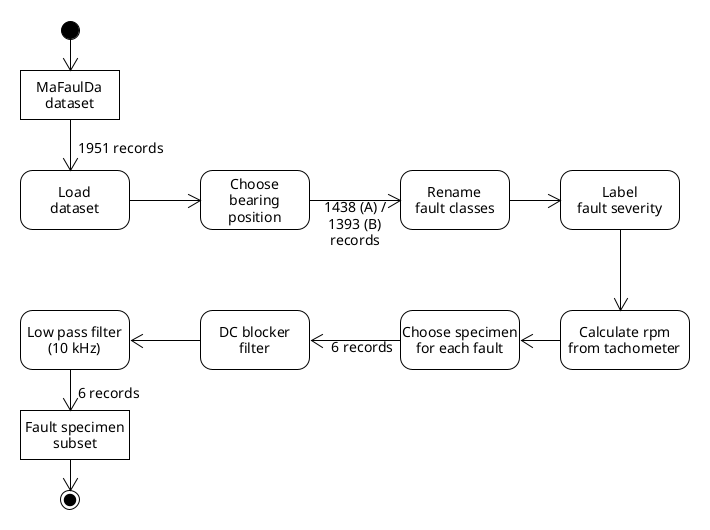
\includegraphics[width=\textwidth]{assets/design/activity-data-exploration.png}
	\caption{Activity diagram of MaFaulDa dataset preprocessing}
	\label{fig:design:mafaulda-preprocessing}
\end{figure}

MaFaulda contains 1951 records labeled with inducted faults of increasing severity. The defects were set up on the machine simulator as is mentioned in the part about datasets. Time series of the triaxial piezoelectric accelerometers in separate files have a sampling frequency of 50 kHz. 

These vibration sensors are placed in two positions. The first placement is around the inner underhang bearing named \emph{A} which is closer to the motor. The second location is around the outer overhang bearing denoted as \emph{B} position.

\subsection{Fault annotations}
The dataset has annotations altogether for 10 classes of faults of which there is 1 class for fault-free baseline operation, 3 classes for shaft defects, 3 classes for inner bearing defects, and 3 for outer bearing defects. Some categories are redundant or irrelevant for a given sensor position. 

Therefore rotor shaft misalignements in vertical and horizontal directions are merged into one joint group. Depending on the chosen bearing position only records having relevant labels are considered. 

This means that fault classification solely concerns bearing in the direct contact and shaft mechanically passing through it. The bearings affect each other, but the effect on the opposite side should appear via a common interconnection shaft. 

In the end, that leaves \textbf{6 types of labels}: baseline, two shaft faults are imbalance and misalignment, and three bearing faults are cage fault, ball fault, and outer race fault. In the step of choosing the accelerometer location records pointing to the other bearing as a source of the malfunction are discarded. Then the next action renames the labels to be better recognizable and unite the same phenomena.

Groups of identified machine defects are additionally characterized by altered masses attached or motor shaft displacement shifts. The set amount is sorted in ascending order separating \textbf{multiple event severities}. However, the count of severity levels is not identical in every group. Levels are hence scaled into the range between zero and one using a min-max scaler. Scaling is applied to classes separately.

The strength of the recorded response by the underlying defect is also dependent on the shaft \textbf{rotational speed}. Speed in rpm is calculated from pulsed speedometer output. It is the average distance between two successive rising edges: 
\begin{ceqn}\begin{align}
\mathrm{rpm} = 60 \;/\; \overline{\Delta t}
\end{align}\end{ceqn}

\textbf{A specimen waveform} is picked from each fault class to illustrate their superficial differences. Recordings are filtered to get one of the highest severity levels and around a mean rotation speed of 2500 rpm (42 Hz)  to see the patterns most pronounced. The baseline class sample is chosen according to fixed rotor speed.


\subsection{Signal filters}
The DC component in the three-dimensional vibration signal is removed by subtracting the global mean. Immediately follows a digital IIR Butterworth \textbf{ low pass filter} of \nth{5} order with cutoff frequency 10 kHz at -3 dB. 

Before the low pass filter usage, the peak at 20 kHz with sideband was present as an unwanted artifact. It could not have been reliably recorded due to the linear frequency response of the sensor up to 10 kHz. At the same time, such frequency is outside the range of any feasible MEMS accelerometer.

\begin{figure}[ht]
    \centering
    \begin{subfigure}[b]{0.44\textwidth}
        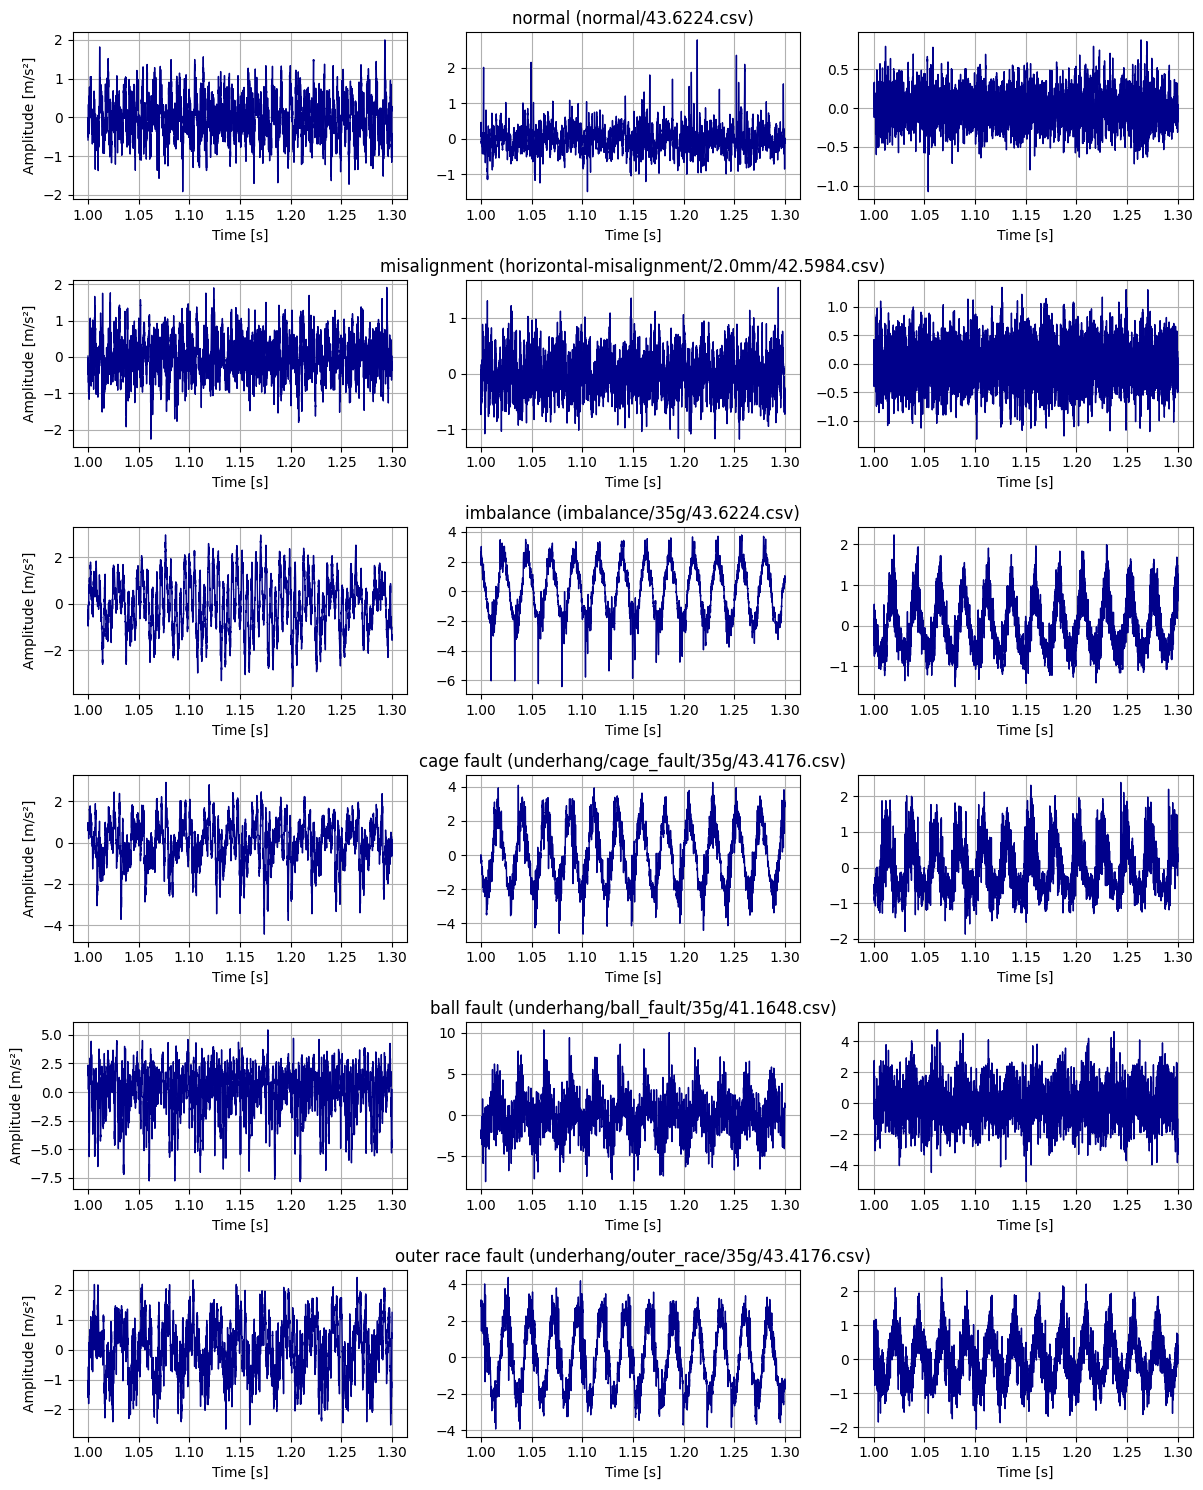
\includegraphics[width=\textwidth]{assets/design/Mafaulda-A-time-waveform.png}
        \caption{Temporal domain waveforms}
        \label{fig:design:fault-temporal-waveform}
    \end{subfigure}
    \hfill
    \begin{subfigure}[b]{0.55\textwidth}
        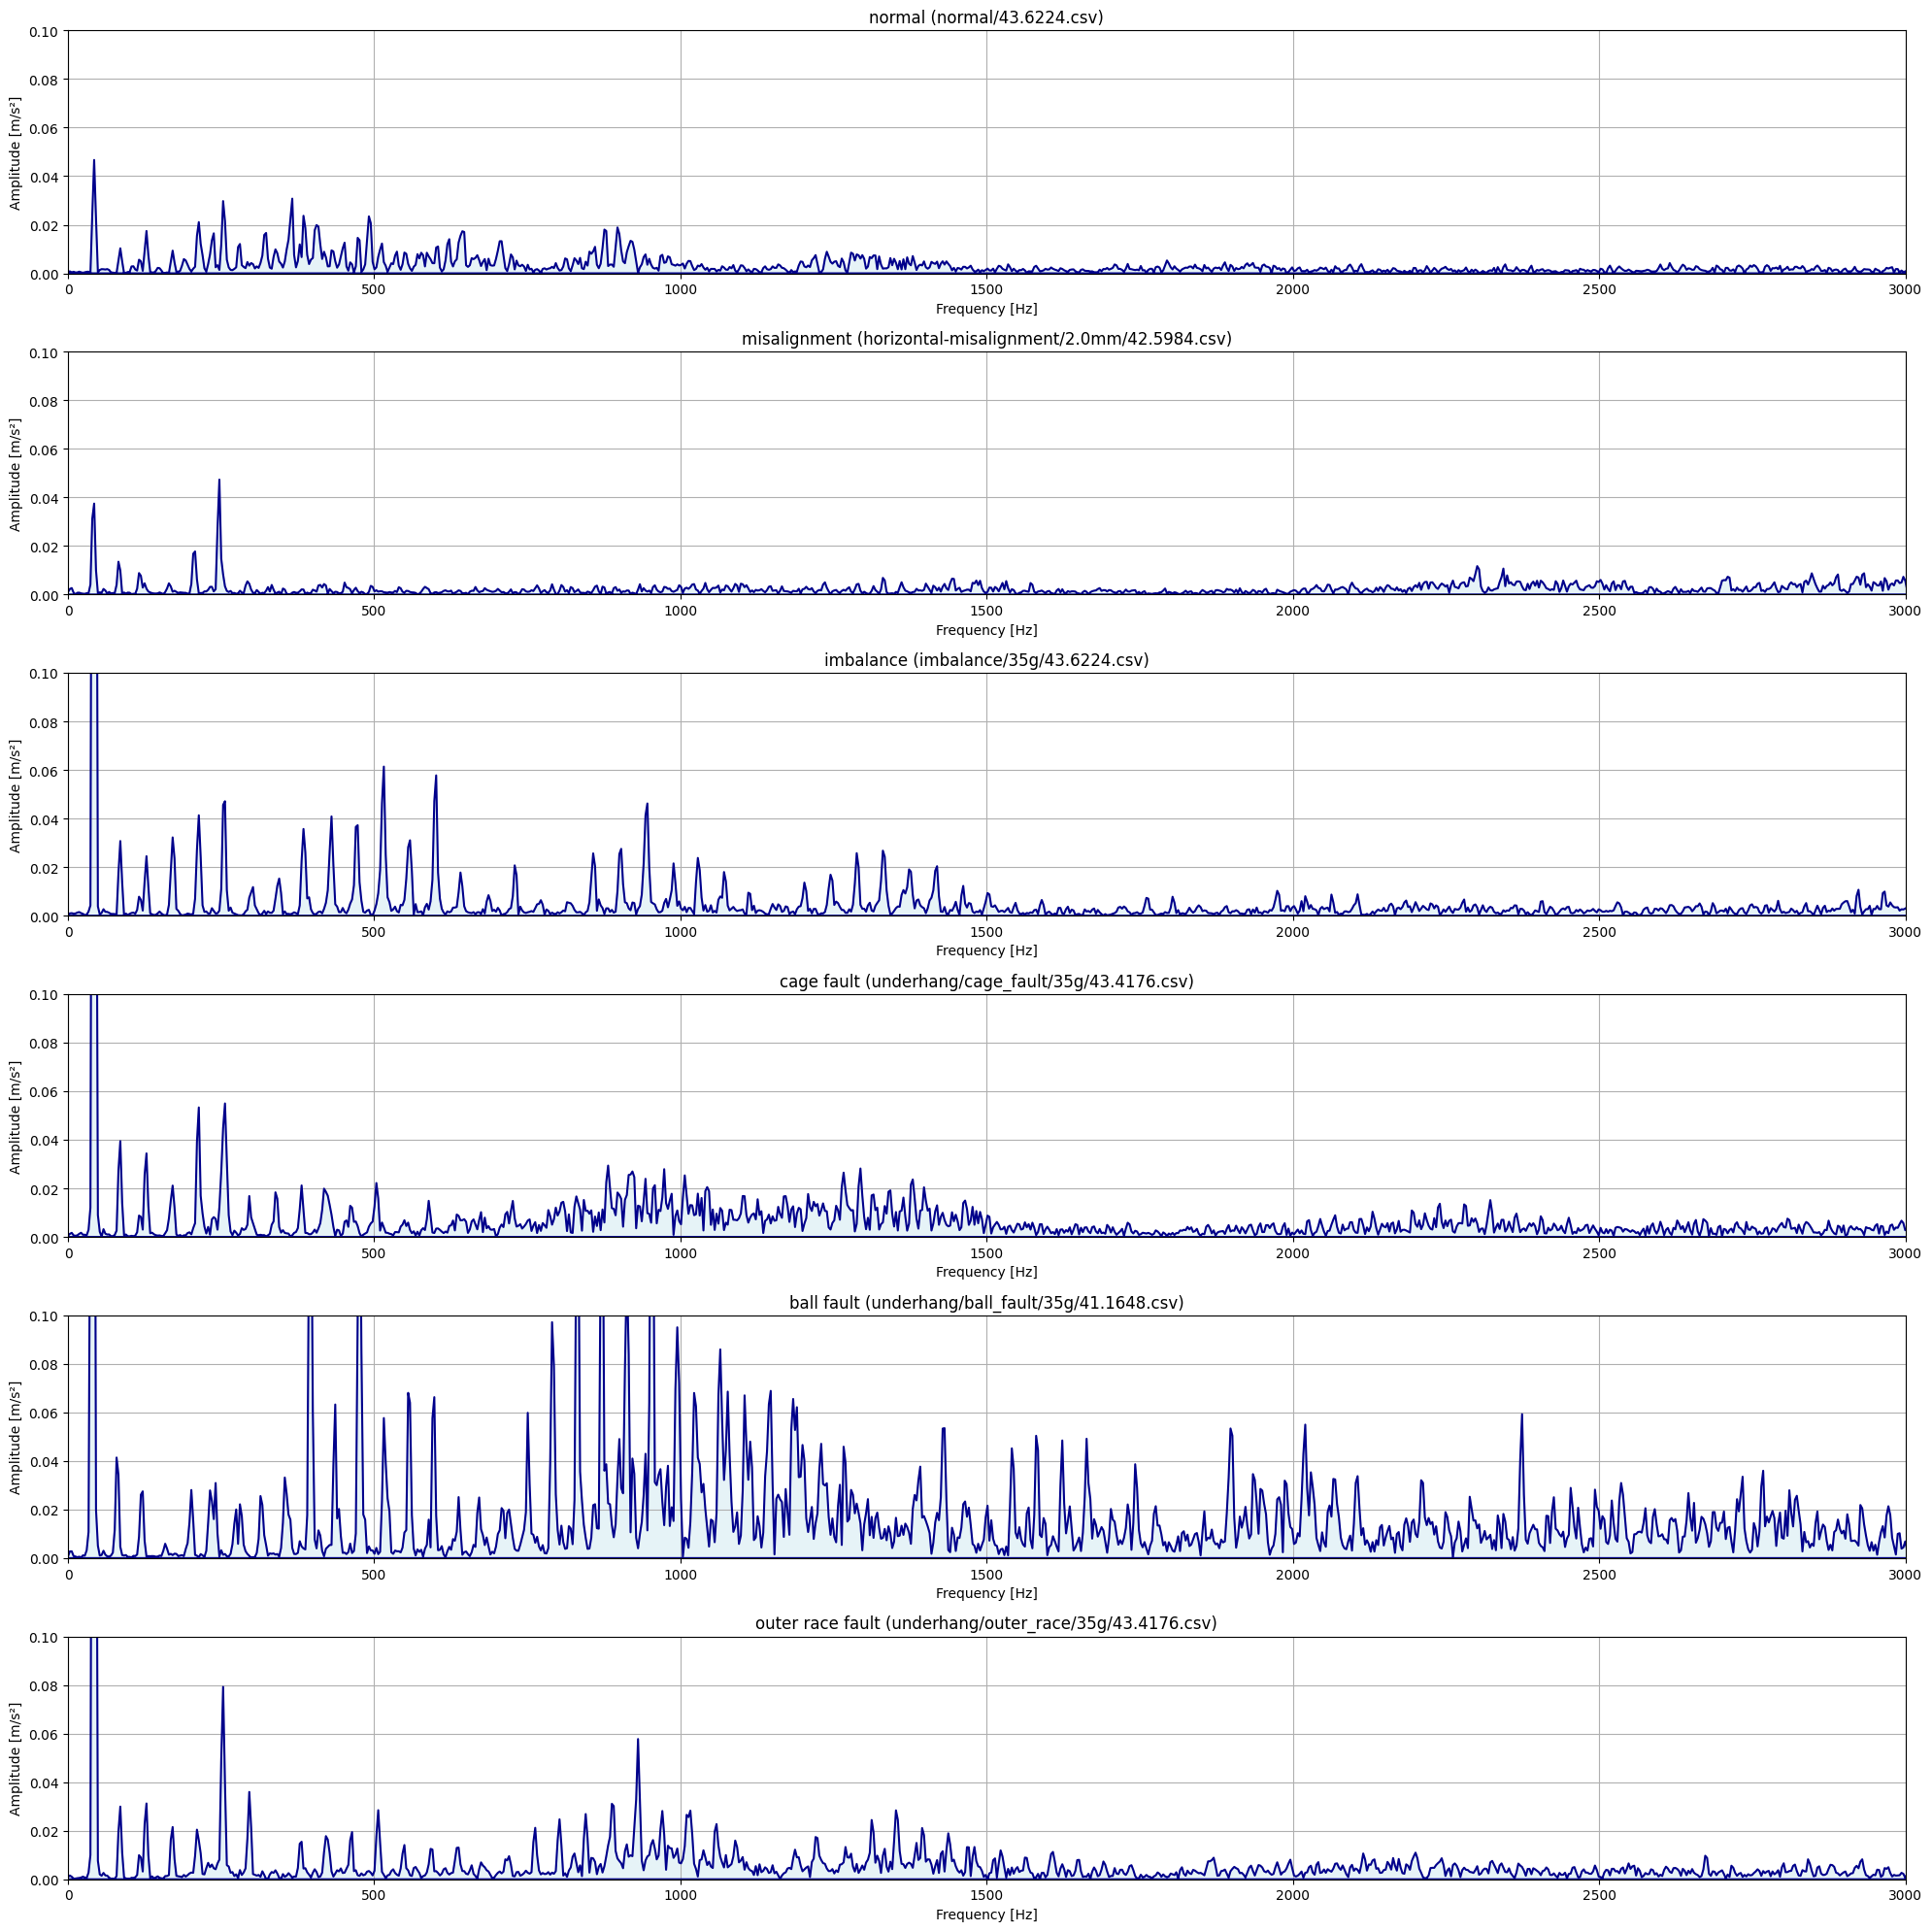
\includegraphics[width=\textwidth]{assets/design/Mafaulda-A-spectrum-Y-axis.png}
        \caption{Spectra in radial direction}
        \label{fig:design:fault-spectral-waveform}
    \end{subfigure} 
    \caption{Signals for each fault category with the highest fault severity at 2500 rpm}
\end{figure}

Temporal domain waveforms of the 300 ms signal slice are shown in the graphs in Figure \ref{fig:design:fault-temporal-waveform}. Subplots for radial, tangential, and axial directions are laid out in columns from left to right. Amplitudes vary with limits from $\pm 3\; \mathrm{m/s}^2$ in baseline and misalignment time series up to $\pm 11\;\mathrm{m/s}^2$ in case of severe bearing faults. 

The frequency spectrum in Figure \ref{fig:design:fault-spectral-waveform} is obtained by FFT and Hann window of length $2^{14}$. The signal chunk represents an uncertainty box with a duration of approximately 328 ms and a spectral resolution of little over 3 Hz. The graph has been cropped in both axes to make the most important peaks visible.


\subsection{Statistical tests}
%TODO boxplot in featue selection
%TODO images of machines
%TODO


\subsection{Feature extraction}
%TODO - activity diagram, implementation and value counts
\begin{table}[ht]
\renewcommand{\arraystretch}{1.2}
\begin{tabular}{rrrrrllll}
\cline{1-5}
\multicolumn{1}{|l|}{\multirow{2}{*}{\textbf{Fault}}} & \multicolumn{2}{l|}{\textbf{All rotational speeds}}                                               & \multicolumn{2}{l|}{\textbf{\begin{tabular}[c]{@{}l@{}}Selected rotational speeds \\ 2500 $\pm$ 500 rpm\end{tabular}}} &                               &                               &                               &                               \\ \cline{2-5}
\multicolumn{1}{|l|}{}                                & \multicolumn{1}{l|}{\textbf{Inner bearing (A)}} & \multicolumn{1}{l|}{\textbf{Outer bearing (B)}} & \multicolumn{1}{l|}{\textbf{Inner bearing (A)}}            & \multicolumn{1}{l|}{\textbf{Outer bearing (B)}}           &                               &                               &                               &                               \\ \cline{1-5}
\multicolumn{1}{|r|}{\textbf{normal}}                 & \multicolumn{1}{r|}{49 (3\%)}                   & \multicolumn{1}{r|}{49 (4\%)}                   & \multicolumn{1}{r|}{16 (3\%)}                              & \multicolumn{1}{r|}{16 (3\%)}                             &                               &                               &                               &                               \\ \cline{1-5}
\multicolumn{1}{|r|}{\textbf{misalignment}}           & \multicolumn{1}{r|}{498 (35\%)}                 & \multicolumn{1}{r|}{498 (36\%)}                 & \multicolumn{1}{r|}{173 (34\%)}                            & \multicolumn{1}{r|}{173 (36\%)}                           &                               &                               &                               &                               \\ \cline{1-5}
\multicolumn{1}{|r|}{\textbf{imbalance}}              & \multicolumn{1}{r|}{333 (23\%)}                 & \multicolumn{1}{r|}{333 (24\%)}                 & \multicolumn{1}{r|}{118 (23\%)}                            & \multicolumn{1}{r|}{118 (25\%)}                           &                               &                               &                               &                               \\ \cline{1-5}
\multicolumn{1}{|r|}{\textbf{cage fault}}             & \multicolumn{1}{r|}{188 (13\%)}                 & \multicolumn{1}{r|}{188 (13\%)}                 & \multicolumn{1}{r|}{67 (13\%)}                             & \multicolumn{1}{r|}{69 (14\%)}                            &                               &                               &                               &                               \\ \cline{1-5}
\multicolumn{1}{|r|}{\textbf{ball fault}}             & \multicolumn{1}{r|}{186 (13\%)}                 & \multicolumn{1}{r|}{137 (10\%)}                 & \multicolumn{1}{r|}{61 (12\%)}                             & \multicolumn{1}{r|}{34 (7\%)}                             &                               &                               &                               &                               \\ \cline{1-5}
\multicolumn{1}{|r|}{\textbf{outer race fault}}       & \multicolumn{1}{r|}{184 (13\%)}                 & \multicolumn{1}{r|}{188 (13\%)}                 & \multicolumn{1}{r|}{69 (14\%)}                             & \multicolumn{1}{r|}{68 (14\%)}                            &                               &                               &                               &                               \\ \cline{1-5}
\multicolumn{1}{|r|}{\textbf{Total}}                  & \multicolumn{1}{r|}{1438}                       & \multicolumn{1}{r|}{1393}                       & \multicolumn{1}{r|}{504}                                   & \multicolumn{1}{r|}{478}                                  & \multicolumn{1}{r}{\textbf{}} & \multicolumn{1}{r}{\textbf{}} & \multicolumn{1}{r}{\textbf{}} & \multicolumn{1}{r}{\textbf{}} \\ \cline{1-5}
\textbf{}                                             &                                                 &                                                 &                                                            &                                                           & \multicolumn{1}{r}{}          & \multicolumn{1}{r}{}          & \multicolumn{1}{r}{}          & \multicolumn{1}{r}{}          \\
\textbf{}                                             &                                                 &                                                 &                                                            &                                                           & \multicolumn{1}{r}{}          & \multicolumn{1}{r}{}          & \multicolumn{1}{r}{}          & \multicolumn{1}{r}{}          \\
\textbf{}                                             &                                                 &                                                 &                                                            &                                                           & \multicolumn{1}{r}{}          & \multicolumn{1}{r}{}          & \multicolumn{1}{r}{}          & \multicolumn{1}{r}{}          \\
\textbf{}                                             &                                                 &                                                 &                                                            &                                                           & \multicolumn{1}{r}{}          & \multicolumn{1}{r}{}          & \multicolumn{1}{r}{}          & \multicolumn{1}{r}{}          \\
                                                      &                                                 &                                                 &                                                            &                                                           & \multicolumn{1}{r}{}          & \multicolumn{1}{r}{}          & \multicolumn{1}{r}{}          & \multicolumn{1}{r}{}          \\
                                                      &                                                 &                                                 &                                                            &                                                           & \multicolumn{1}{r}{}          & \multicolumn{1}{r}{}          & \multicolumn{1}{r}{}          & \multicolumn{1}{r}{}         
\end{tabular}
\end{table}



\begin{table}[ht]
\renewcommand{\arraystretch}{1.2}
\begin{tabular}{rrrrrrrrr}
\cline{1-5}
\multicolumn{1}{|l|}{\multirow{2}{*}{\textbf{\begin{tabular}[c]{@{}l@{}}Anomaly\\ 60\% severity\end{tabular}}}} & \multicolumn{2}{l|}{\textbf{All rotational speeds}}                                               & \multicolumn{2}{l|}{\textbf{\begin{tabular}[c]{@{}l@{}}Selected rotational speeds \\ 2500 $\pm$ 500 rpm\end{tabular}}} & \multicolumn{1}{l}{} & \multicolumn{1}{l}{} & \multicolumn{1}{l}{} & \multicolumn{1}{l}{} \\ \cline{2-5}
\multicolumn{1}{|l|}{}                                                                                          & \multicolumn{1}{l|}{\textbf{Inner bearing (A)}} & \multicolumn{1}{l|}{\textbf{Outer bearing (B)}} & \multicolumn{1}{l|}{\textbf{Inner bearing (A)}}            & \multicolumn{1}{l|}{\textbf{Outer bearing (B)}}           & \multicolumn{1}{l}{} & \multicolumn{1}{l}{} & \multicolumn{1}{l}{} & \multicolumn{1}{l}{} \\ \cline{1-5}
\multicolumn{1}{|r|}{\textbf{False}}                                                                            & \multicolumn{1}{r|}{837 (58\%)}                 & \multicolumn{1}{r|}{831 (60\%)}                 & \multicolumn{1}{r|}{375 (74\%)}                            & \multicolumn{1}{r|}{354 (74\%)}                           & \multicolumn{1}{l}{} & \multicolumn{1}{l}{} & \multicolumn{1}{l}{} & \multicolumn{1}{l}{} \\ \cline{1-5}
\multicolumn{1}{|r|}{\textbf{True}}                                                                             & \multicolumn{1}{r|}{601 (42\%)}                 & \multicolumn{1}{r|}{562 (40\%)}                 & \multicolumn{1}{r|}{129 (26\%)}                            & \multicolumn{1}{r|}{124 (26\%)}                           & \multicolumn{1}{l}{} & \multicolumn{1}{l}{} & \multicolumn{1}{l}{} & \multicolumn{1}{l}{} \\ \cline{1-5}
\multicolumn{1}{|r|}{\textbf{Total}}                                                                                 & \multicolumn{1}{r|}{1438}                       & \multicolumn{1}{r|}{1393}                       & \multicolumn{1}{r|}{504}                                   & \multicolumn{1}{r|}{478}                                  & \textbf{}            & \textbf{}            & \textbf{}            & \textbf{}            \\ \cline{1-5}
\textbf{}                                                                                                       &                                                 &                                                 &                                                            &                                                           &                      &                      &                      &                      \\
\textbf{}                                                                                                       & \textbf{}                                       & \textbf{}                                       & \textbf{}                                                  & \textbf{}                                                 & \textbf{}            & \textbf{}            & \textbf{}            & \textbf{}            \\
\textbf{}                                                                                                       &                                                 &                                                 &                                                            &                                                           &                      &                      &                      &                      \\
\textbf{}                                                                                                       &                                                 &                                                 &                                                            &                                                           &                      &                      &                      &                      \\
                                                                                                                &                                                 &                                                 &                                                            &                                                           &                      &                      &                      &                      \\
                                                                                                                &                                                 &                                                 &                                                            &                                                           &                      &                      &                      &                     
\end{tabular}
\end{table}


\begin{table}[ht]
\renewcommand{\arraystretch}{1.2}
\begin{tabular}{rrrrrrrrr}
\cline{1-5}
\multicolumn{1}{|l|}{\multirow{2}{*}{\textbf{\begin{tabular}[c]{@{}l@{}}Anomaly\\ 90\% severity\end{tabular}}}} & \multicolumn{2}{l|}{\textbf{All rotational speeds}}                                               & \multicolumn{2}{l|}{\textbf{\begin{tabular}[c]{@{}l@{}}Selected rotational speeds \\ 2500 $\pm$ 500 rpm\end{tabular}}} & \multicolumn{1}{l}{} & \multicolumn{1}{l}{} & \multicolumn{1}{l}{} & \multicolumn{1}{l}{} \\ \cline{2-5}
\multicolumn{1}{|l|}{}                                                                                          & \multicolumn{1}{l|}{\textbf{Inner bearing (A)}} & \multicolumn{1}{l|}{\textbf{Outer bearing (B)}} & \multicolumn{1}{l|}{\textbf{Inner bearing (A)}}            & \multicolumn{1}{l|}{\textbf{Outer bearing (B)}}           & \multicolumn{1}{l}{} & \multicolumn{1}{l}{} & \multicolumn{1}{l}{} & \multicolumn{1}{l}{} \\ \cline{1-5}
\multicolumn{1}{|r|}{\textbf{False}}                                                                            & \multicolumn{1}{r|}{837 (58\%)}                 & \multicolumn{1}{r|}{831 (60\%)}                 & \multicolumn{1}{r|}{375 (74\%)}                            & \multicolumn{1}{r|}{354 (74\%)}                           & \multicolumn{1}{l}{} & \multicolumn{1}{l}{} & \multicolumn{1}{l}{} & \multicolumn{1}{l}{} \\ \cline{1-5}
\multicolumn{1}{|r|}{\textbf{True}}                                                                             & \multicolumn{1}{r|}{601 (42\%)}                 & \multicolumn{1}{r|}{562 (40\%)}                 & \multicolumn{1}{r|}{129 (26\%)}                            & \multicolumn{1}{r|}{124 (26\%)}                           & \multicolumn{1}{l}{} & \multicolumn{1}{l}{} & \multicolumn{1}{l}{} & \multicolumn{1}{l}{} \\ \cline{1-5}
\multicolumn{1}{|r|}{\textbf{Total}}                                                                                 & \multicolumn{1}{r|}{1438}                       & \multicolumn{1}{r|}{1393}                       & \multicolumn{1}{r|}{504}                                   & \multicolumn{1}{r|}{478}                                  & \textbf{}            & \textbf{}            & \textbf{}            & \textbf{}            \\ \cline{1-5}
\textbf{}                                                                                                       &                                                 &                                                 &                                                            &                                                           &                      &                      &                      &                      \\
\textbf{}                                                                                                       & \textbf{}                                       & \textbf{}                                       & \textbf{}                                                  & \textbf{}                                                 & \textbf{}            & \textbf{}            & \textbf{}            & \textbf{}            \\
\textbf{}                                                                                                       &                                                 &                                                 &                                                            &                                                           &                      &                      &                      &                      \\
\textbf{}                                                                                                       &                                                 &                                                 &                                                            &                                                           &                      &                      &                      &                      \\
                                                                                                                &                                                 &                                                 &                                                            &                                                           &                      &                      &                      &                      \\
                                                                                                                &                                                 &                                                 &                                                            &                                                           &                      &                      &                      &                     
\end{tabular}
\end{table}


\section{Feature relevance}

\begin{figure}[ht]
    \centering
    \begin{subfigure}[b]{0.49\textwidth}
        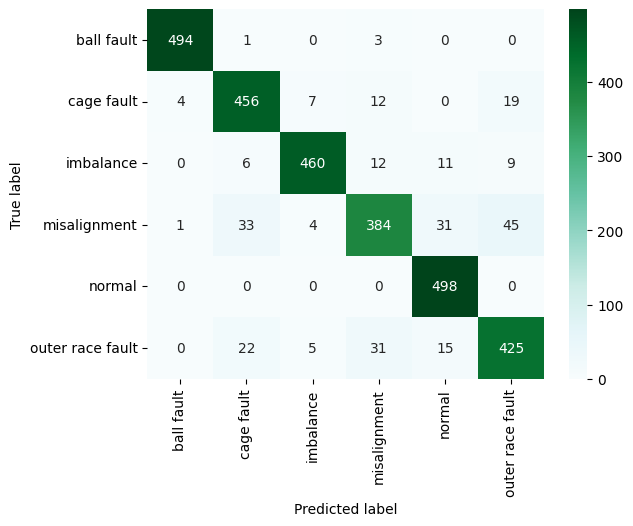
\includegraphics[width=\textwidth]{assets/design/kNN-temporal-confusion-matrix-fault.png}
        \caption{Prediction for 6 fault classes in testing set with temporal domain features}
    \end{subfigure}
    \hfill
    \begin{subfigure}[b]{0.49\textwidth}
        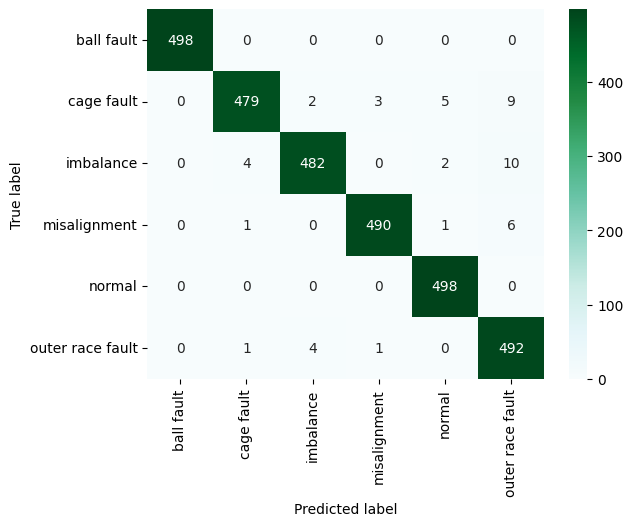
\includegraphics[width=\textwidth]{assets/design/kNN-spectral-confusion-matrix-fault.png}
        \caption{Prediction for 6 fault classes in testing set with spectral domain features}
    \end{subfigure}
    \begin{subfigure}[b]{0.49\textwidth}
        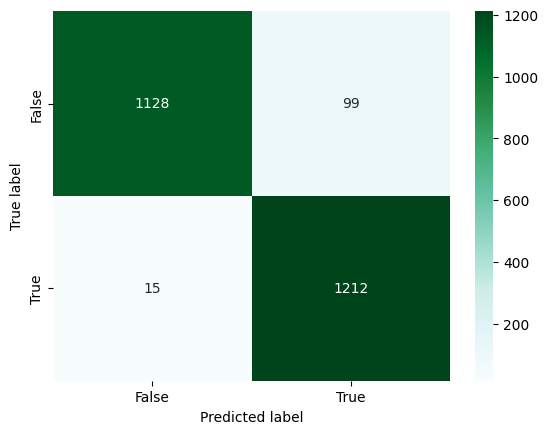
\includegraphics[width=\textwidth]{assets/design/kNN-temporal-confusion-matrix-anomaly90.png}
        \caption{Prediction of high severity anomalies in testing set with temporal domain features}
    \end{subfigure}
    \hfill
    \begin{subfigure}[b]{0.49\textwidth}
        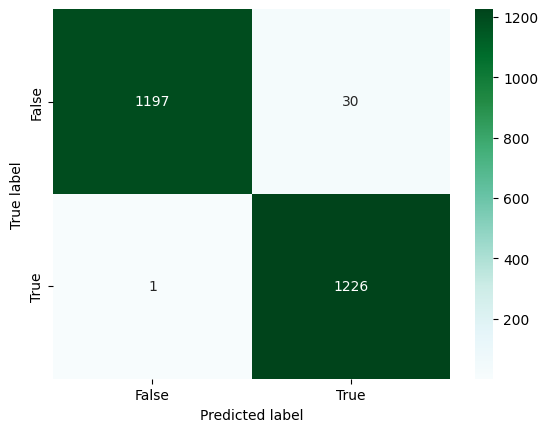
\includegraphics[width=\textwidth]{assets/design/kNN-spectral-confusion-matrix-anomaly90.png}
        \caption{Prediction of high severity anomalies in testing set with spectral domain features}
    \end{subfigure}
    \caption{Confusion matrix of batch kNN algorithm predictions in temporal and spectral domain for two predicted variables measured on inner bearing.}
\end{figure}


\begin{figure}[ht]
    \centering
    \begin{subfigure}[b]{\textwidth}
        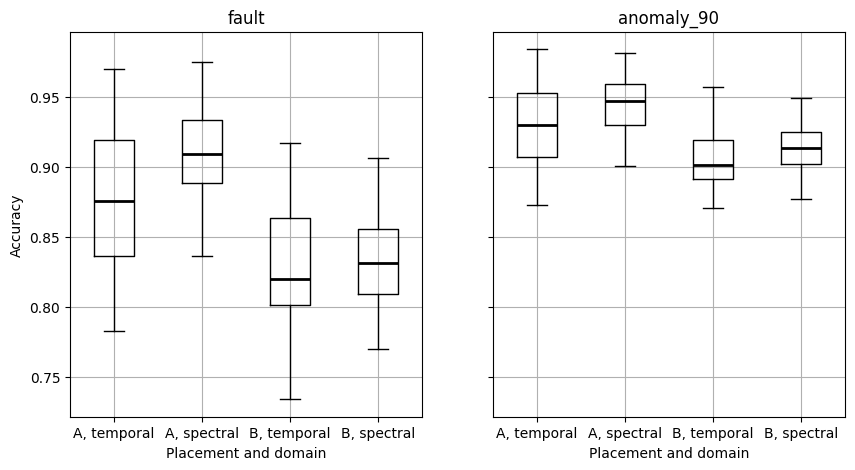
\includegraphics[width=\textwidth]{assets/design/kNN-3-features-combinations-train.png}
        \caption{Testing set}
    \end{subfigure}
    \hfill
    \begin{subfigure}[b]{\textwidth}
        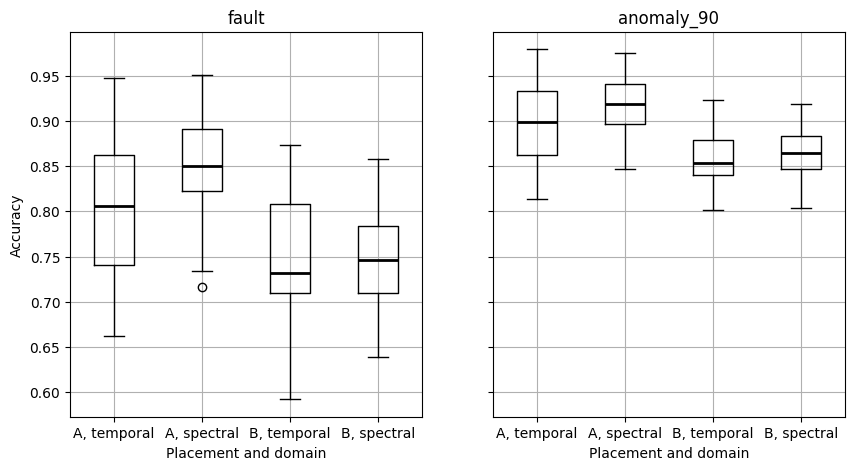
\includegraphics[width=\textwidth]{assets/design/kNN-3-features-combinations-test.png}
        \caption{Training set}
    \end{subfigure}
    \caption{Range of prediction accuracy in all kNN models with subset of 3 features. Subplots show three different predicted variables.}
\end{figure}


\begin{figure}[ht]
    \centering
    \begin{subfigure}[b]{\textwidth}
        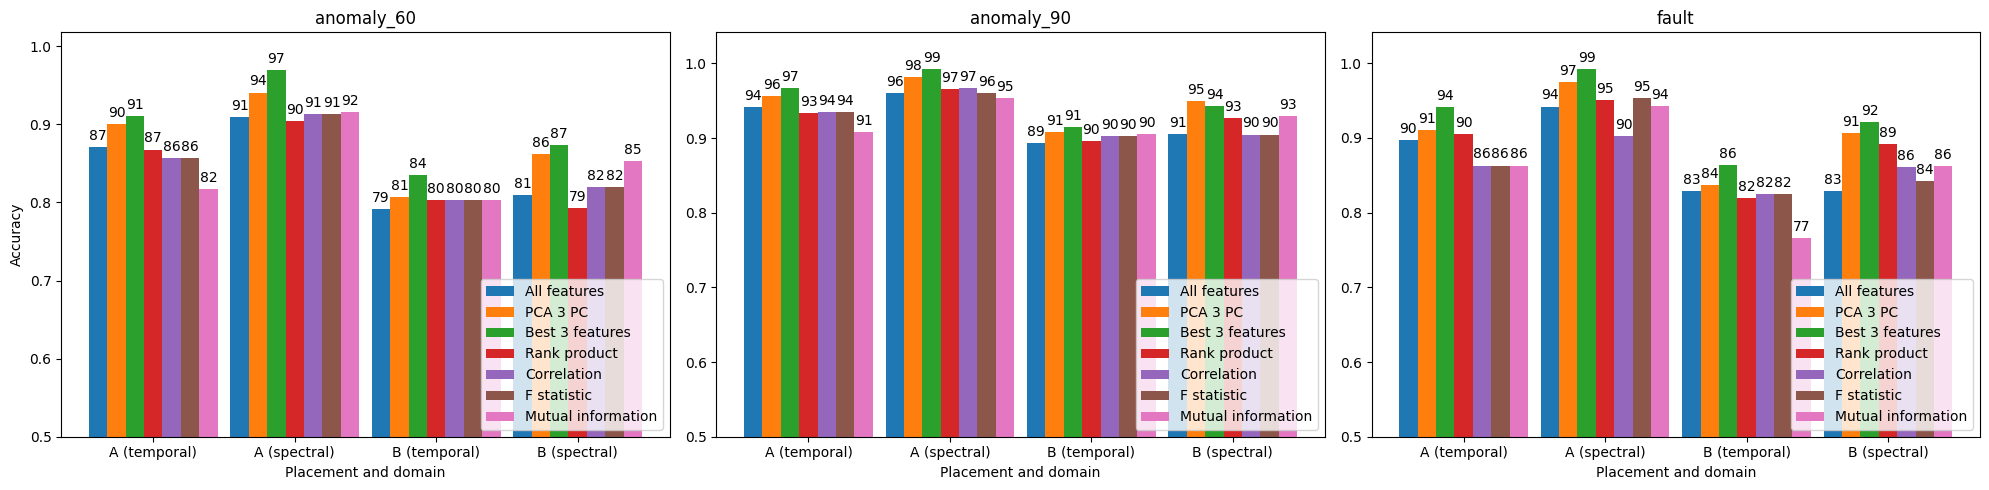
\includegraphics[width=\textwidth]{assets/design/kNN-feature-selection-predictions-train}
        \caption{Testing set}
    \end{subfigure}
    \hfill
    \begin{subfigure}[b]{\textwidth}
        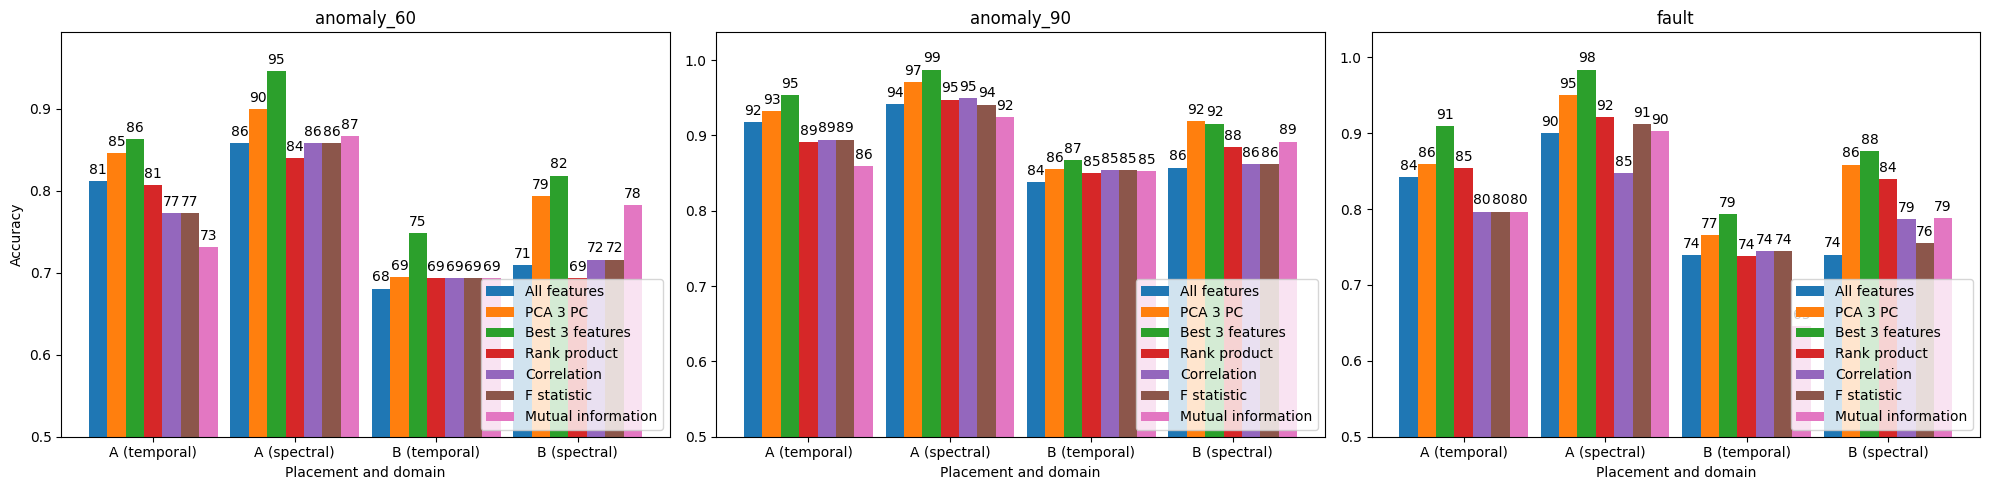
\includegraphics[width=\textwidth]{assets/design/kNN-feature-selection-predictions-test}
        \caption{Training set}
    \end{subfigure} 
    \caption{Batch kNN algorithm prediction accuracy with various feature sets.}
\end{figure}

% Number of neighbors (graphs)


\section{Online kNN model}

\begin{figure}[ht]
    \centering
    \begin{subfigure}[b]{0.49\textwidth}
        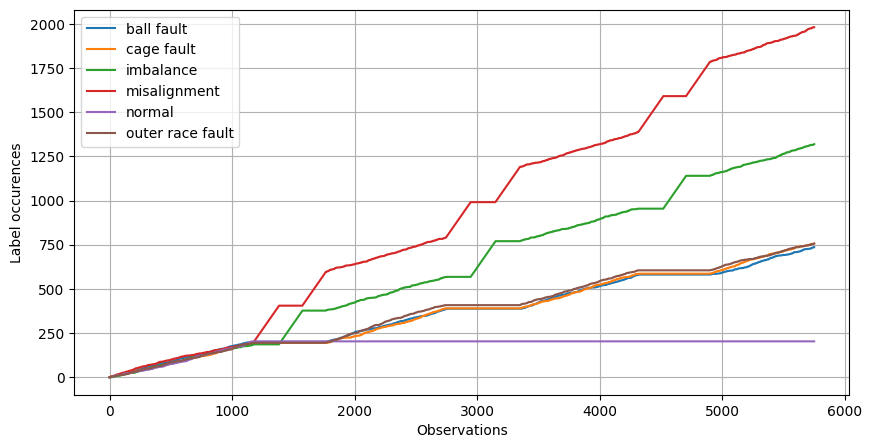
\includegraphics[width=\textwidth]{assets/design/Online-event-ordering-fault-train.png}
        \caption{Training set and fault as predicted variable}
    \end{subfigure}
    \hfill
    \begin{subfigure}[b]{0.49\textwidth}
        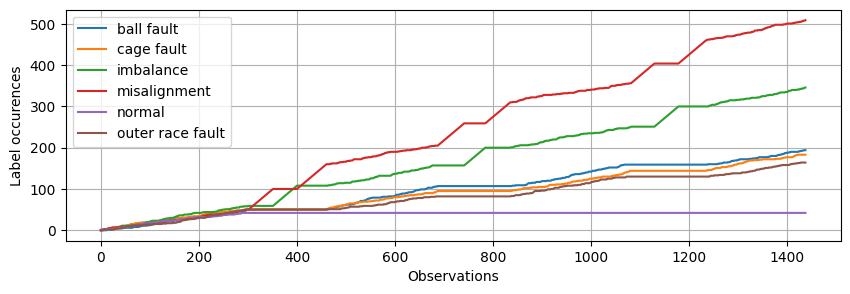
\includegraphics[width=\textwidth]{assets/design/Online-event-ordering-fault-test.png}
        \caption{Testing set and fault as predicted variable}
    \end{subfigure}
    \begin{subfigure}[b]{0.49\textwidth}
        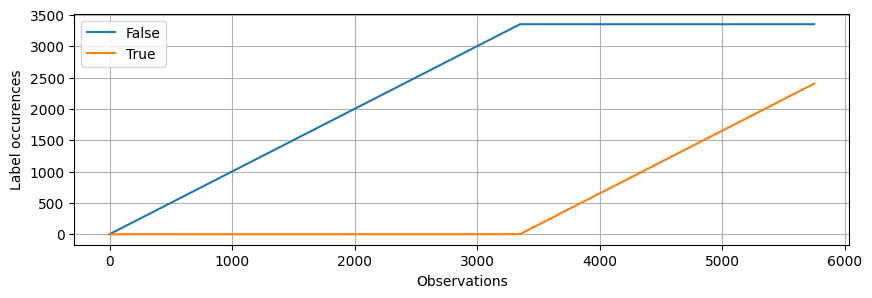
\includegraphics[width=\textwidth]{assets/design/Online-event-ordering-anomaly60-train.png}
        \caption{Training set and medium anomaly severity as predicted variable}
    \end{subfigure}
    \hfill
    \begin{subfigure}[b]{0.49\textwidth}
        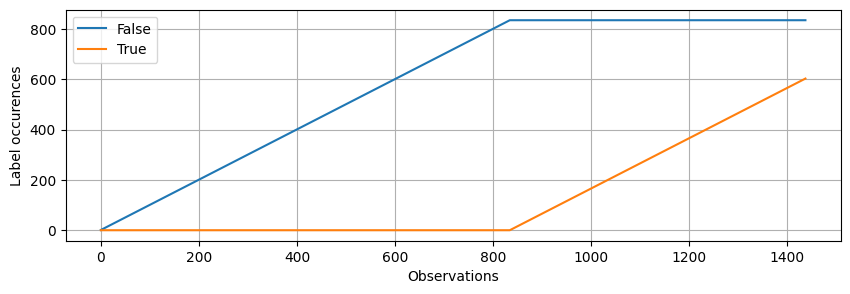
\includegraphics[width=\textwidth]{assets/design/Online-event-ordering-anomaly60-test.png}
        \caption{Training set and medium anomaly severity as predicted variable}
    \end{subfigure}
    \caption{Label order in progressive valuation}
\end{figure}


\begin{figure}[ht]
    \centering
    \begin{subfigure}[b]{0.49\textwidth}
        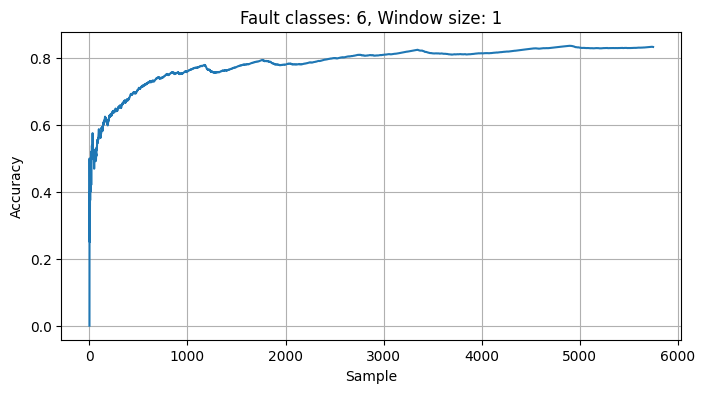
\includegraphics[width=\textwidth]{assets/design/gradual-learning-temporal-domain-fault.png}
        \caption{}
    \end{subfigure}
    \hfill
    \begin{subfigure}[b]{0.49\textwidth}
        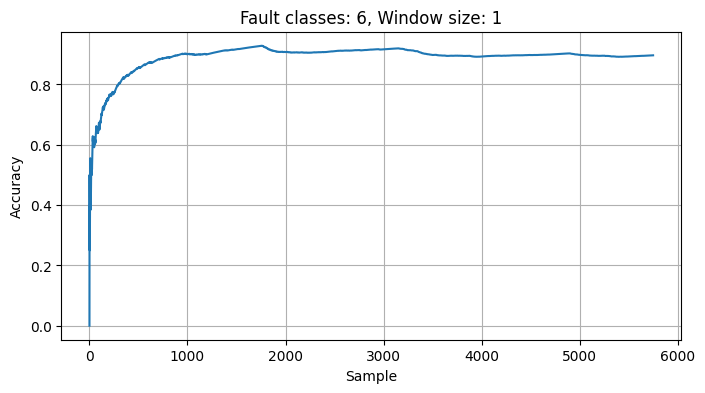
\includegraphics[width=\textwidth]{assets/design/gradual-learning-spectral-domain-fault.png}
        \caption{}
    \end{subfigure}
    \begin{subfigure}[b]{0.49\textwidth}
        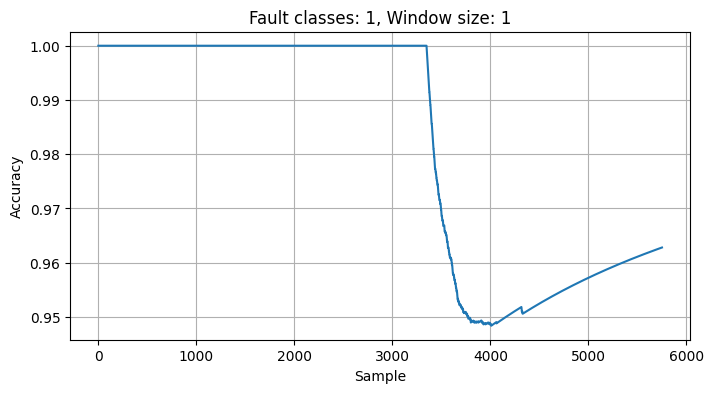
\includegraphics[width=\textwidth]{assets/design/gradual-learning-temporal-domain-anomaly60.png}
        \caption{}
    \end{subfigure}
    \hfill
    \begin{subfigure}[b]{0.49\textwidth}
        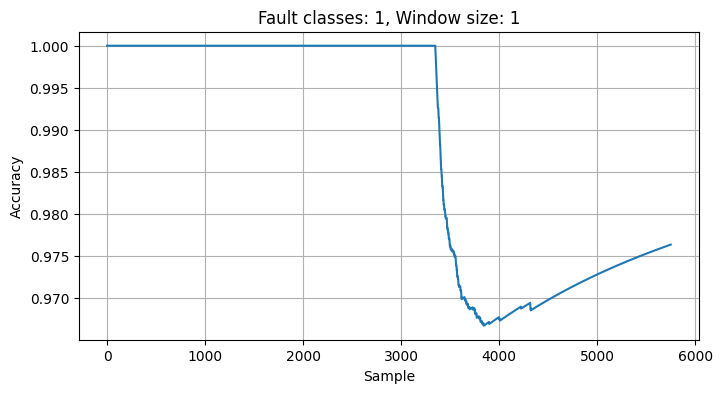
\includegraphics[width=\textwidth]{assets/design/gradual-learning-spectral-domain-anomaly60.png}
        \caption{}
    \end{subfigure}
    \caption{Gradual learning}
\end{figure}


\begin{figure}[ht]
    \centering
    \begin{subfigure}[b]{0.49\textwidth}
        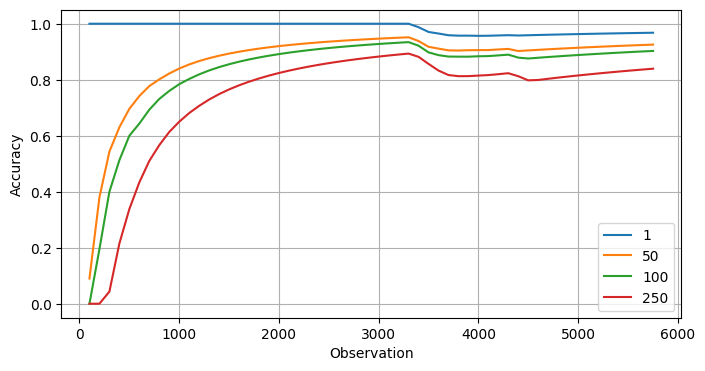
\includegraphics[width=\textwidth]{assets/design/gradual-learning-accuracy-delay-temporal-domain-fault.png}
        \caption{}
    \end{subfigure}
    \hfill
    \begin{subfigure}[b]{0.49\textwidth}
        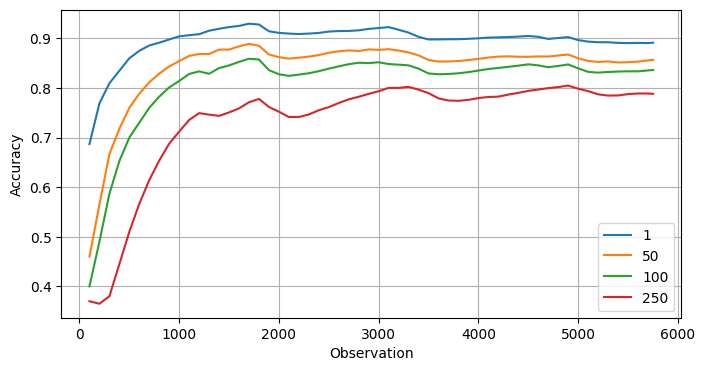
\includegraphics[width=\textwidth]{assets/design/gradual-learning-accuracy-delay-spectral-domain-fault.png}
        \caption{}
    \end{subfigure}
    \begin{subfigure}[b]{0.49\textwidth}
        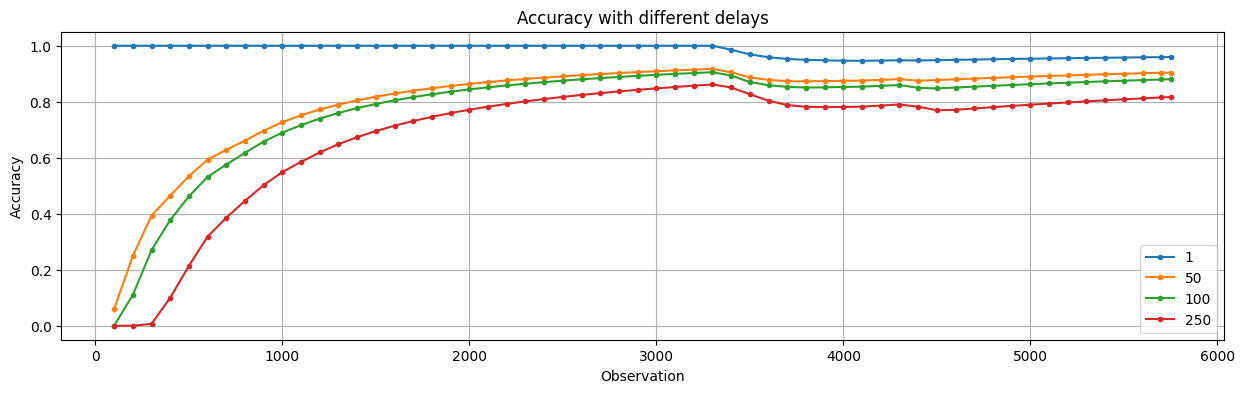
\includegraphics[width=\textwidth]{assets/design/gradual-learning-accuracy-delay-temporal-domain-anomaly60.png}
        \caption{}
    \end{subfigure}
    \hfill
    \begin{subfigure}[b]{0.49\textwidth}
        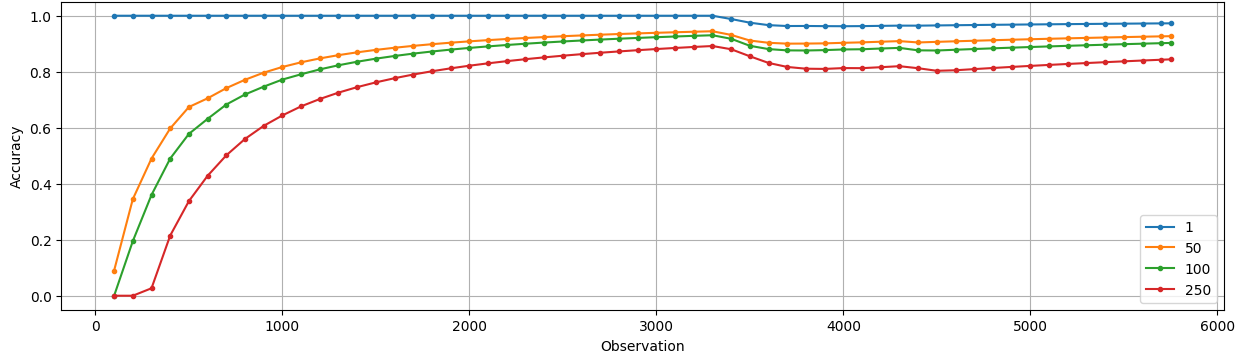
\includegraphics[width=\textwidth]{assets/design/gradual-learning-accuracy-delay-spectral-domain-anomaly60.png}
        \caption{}
    \end{subfigure}
    \caption{Gradual learning accuracy with delay}
\end{figure}



\begin{figure}[ht]
    \centering
    \begin{subfigure}[b]{0.49\textwidth}
        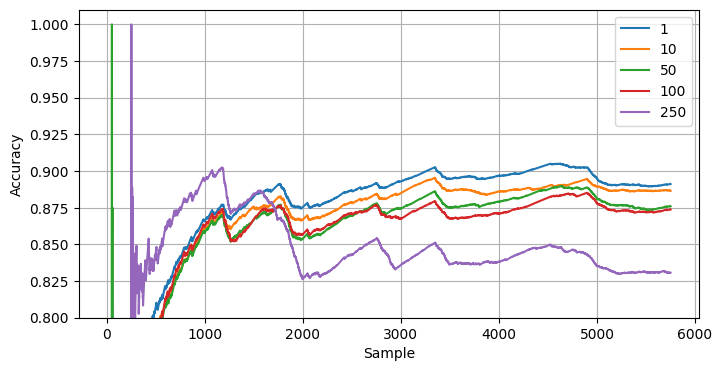
\includegraphics[width=\textwidth]{assets/design/gradual-learning-delay-temporal-domain-fault.png}
        \caption{}
    \end{subfigure}
    \hfill
    \begin{subfigure}[b]{0.49\textwidth}
        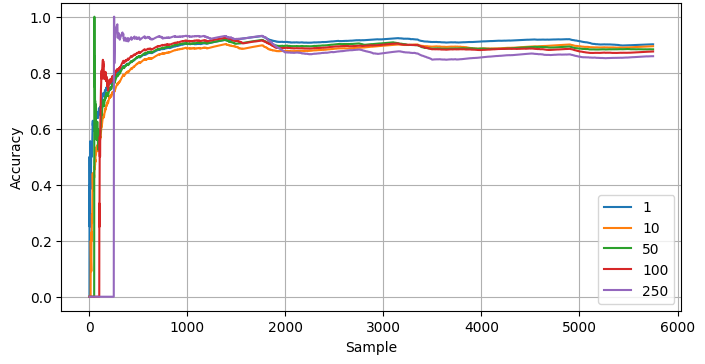
\includegraphics[width=\textwidth]{assets/design/gradual-learning-delay-spectral-domain-fault.png}
        \caption{}
    \end{subfigure}
    \begin{subfigure}[b]{0.49\textwidth}
        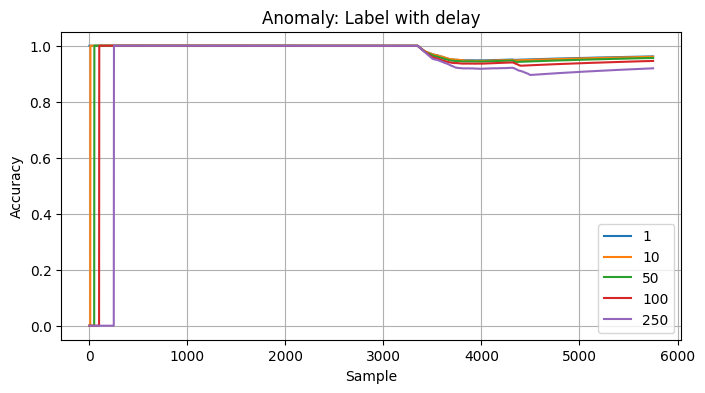
\includegraphics[width=\textwidth]{assets/design/gradual-learning-delay-temporal-domain-anomaly60.png}
        \caption{}
    \end{subfigure}
    \hfill
    \begin{subfigure}[b]{0.49\textwidth}
        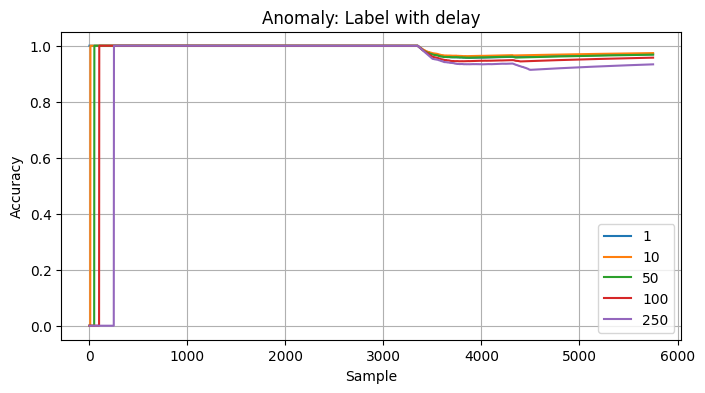
\includegraphics[width=\textwidth]{assets/design/gradual-learning-delay-spectral-domain-anomaly60.png}
        \caption{}
    \end{subfigure}
    \caption{Gradual learning with delay}
\end{figure}



\begin{figure}[ht]
    \centering
    \begin{subfigure}[b]{0.49\textwidth}
        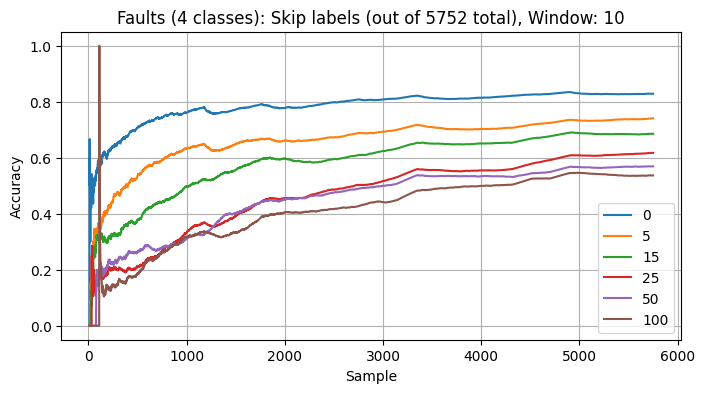
\includegraphics[width=\textwidth]{assets/design/gradual-learning-skip-temporal-domain-fault.png}
        \caption{}
    \end{subfigure}
    \hfill
    \begin{subfigure}[b]{0.49\textwidth}
        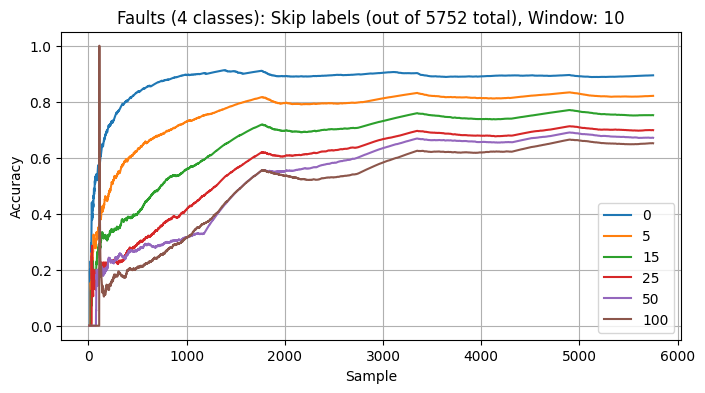
\includegraphics[width=\textwidth]{assets/design/gradual-learning-skip-spectral-domain-fault.png}
        \caption{}
    \end{subfigure}
    \begin{subfigure}[b]{0.49\textwidth}
        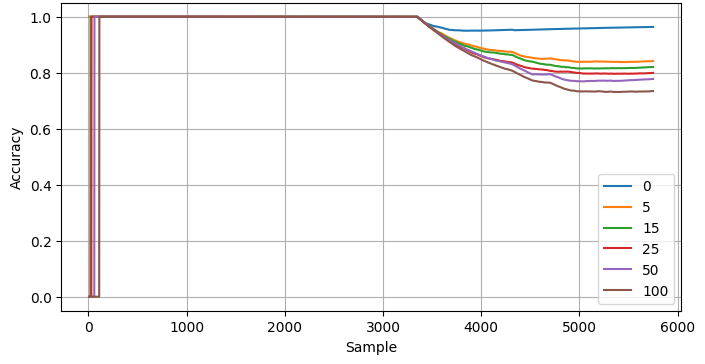
\includegraphics[width=\textwidth]{assets/design/gradual-learning-skip-temporal-domain-anomaly60.png}
        \caption{}
    \end{subfigure}
    \hfill
    \begin{subfigure}[b]{0.49\textwidth}
        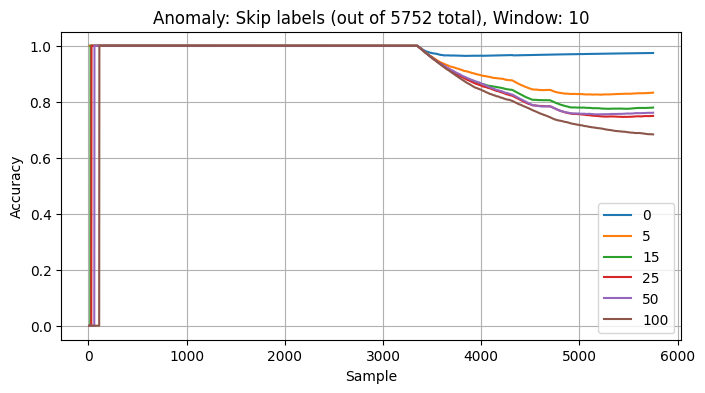
\includegraphics[width=\textwidth]{assets/design/gradual-learning-skip-spectral-domain-anomaly60.png}
        \caption{}
    \end{subfigure}
    \caption{Gradual learning and skip labels}
\end{figure}



\begin{figure}[ht]
    \centering
    \begin{subfigure}[b]{0.49\textwidth}
        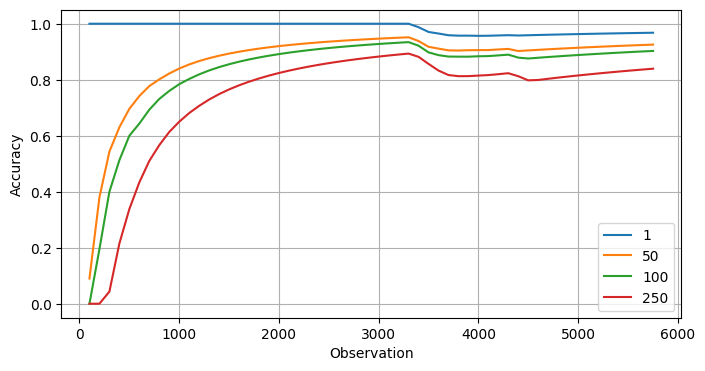
\includegraphics[width=\textwidth]{assets/design/gradual-learning-accuracy-delay-temporal-domain-fault.png}
        \caption{}
    \end{subfigure}
    \hfill
    \begin{subfigure}[b]{0.49\textwidth}
        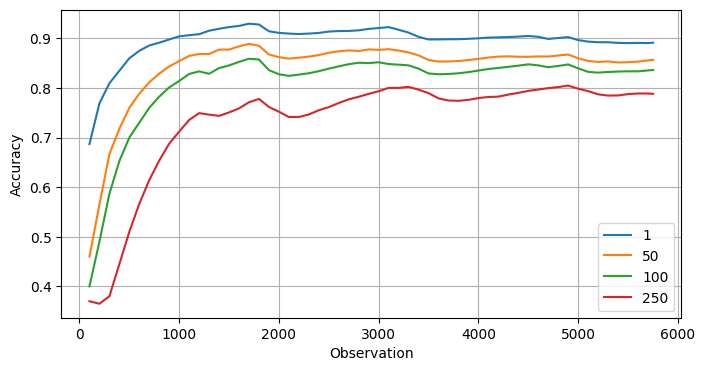
\includegraphics[width=\textwidth]{assets/design/gradual-learning-accuracy-delay-spectral-domain-fault.png}
        \caption{}
    \end{subfigure}
    \begin{subfigure}[b]{0.49\textwidth}
        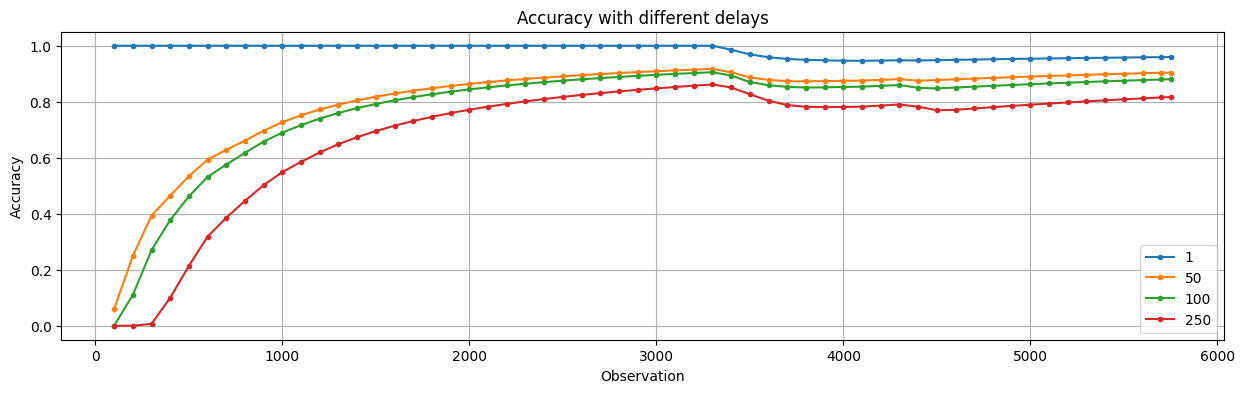
\includegraphics[width=\textwidth]{assets/design/gradual-learning-accuracy-delay-temporal-domain-anomaly60.png}
        \caption{}
    \end{subfigure}
    \hfill
    \begin{subfigure}[b]{0.49\textwidth}
        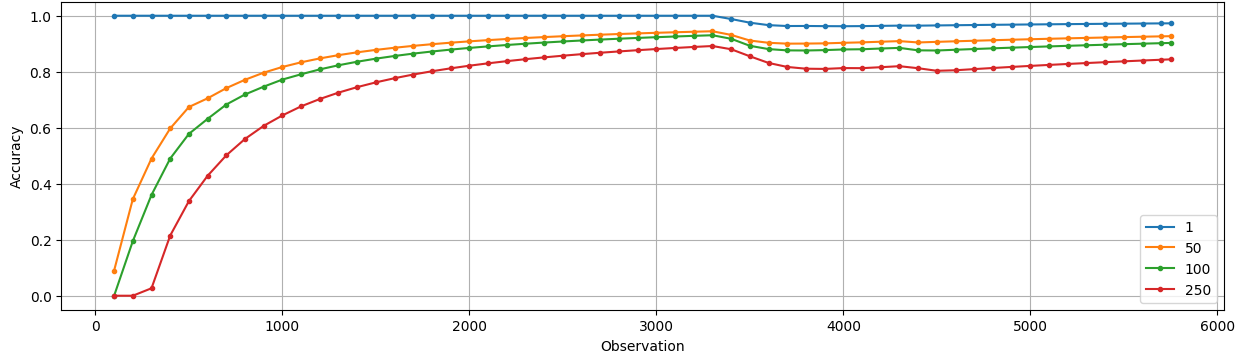
\includegraphics[width=\textwidth]{assets/design/gradual-learning-accuracy-delay-spectral-domain-anomaly60.png}
        \caption{}
    \end{subfigure}
    \caption{Gradual learning accuracy with delay}
\end{figure}



\begin{figure}[ht]
    \centering
    \begin{subfigure}[b]{\textwidth}
        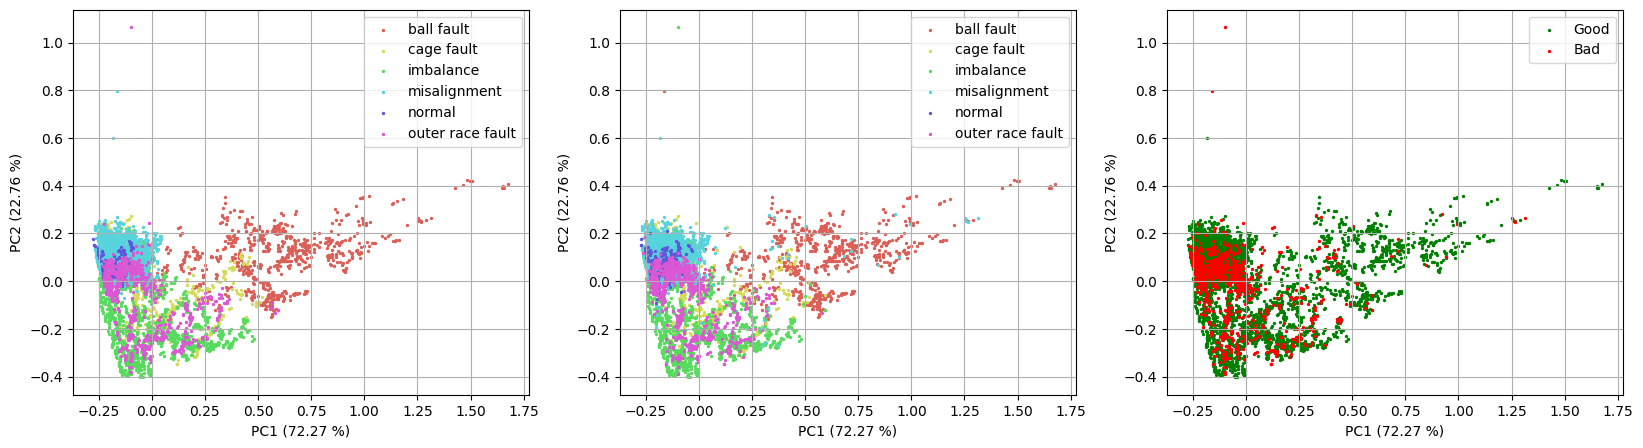
\includegraphics[width=\textwidth]{assets/design/pca-scatter-online-fault-temporal.png}
        \caption{}
    \end{subfigure}
    \hfill
    \begin{subfigure}[b]{\textwidth}
        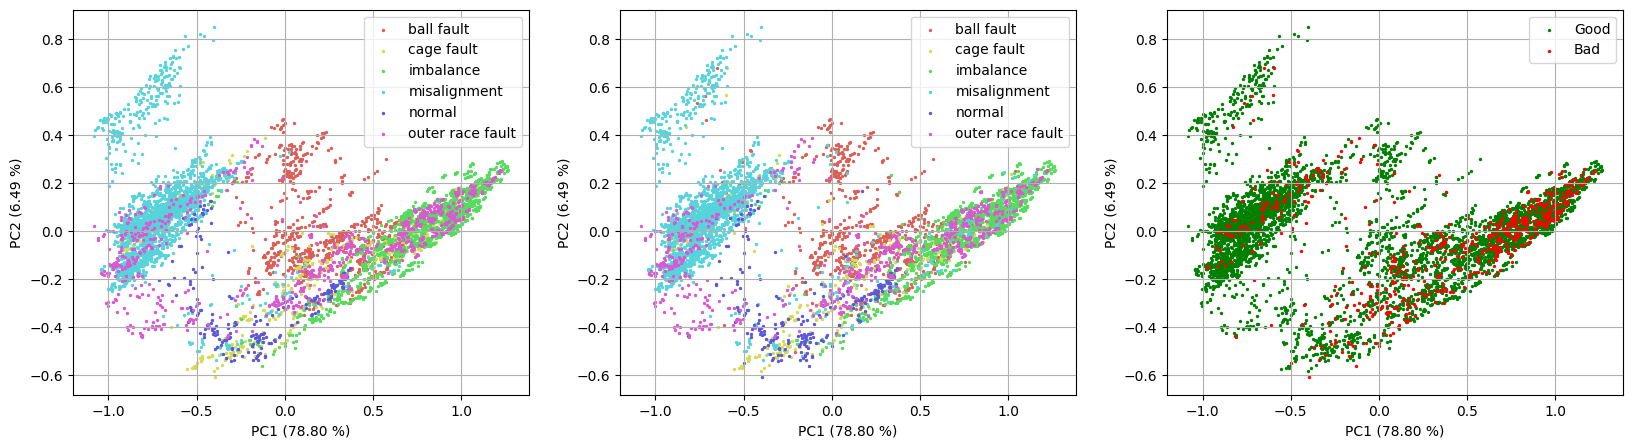
\includegraphics[width=\textwidth]{assets/design/pca-scatter-online-fault-spectral.png}
        \caption{}
    \end{subfigure}
    \begin{subfigure}[b]{\textwidth}
        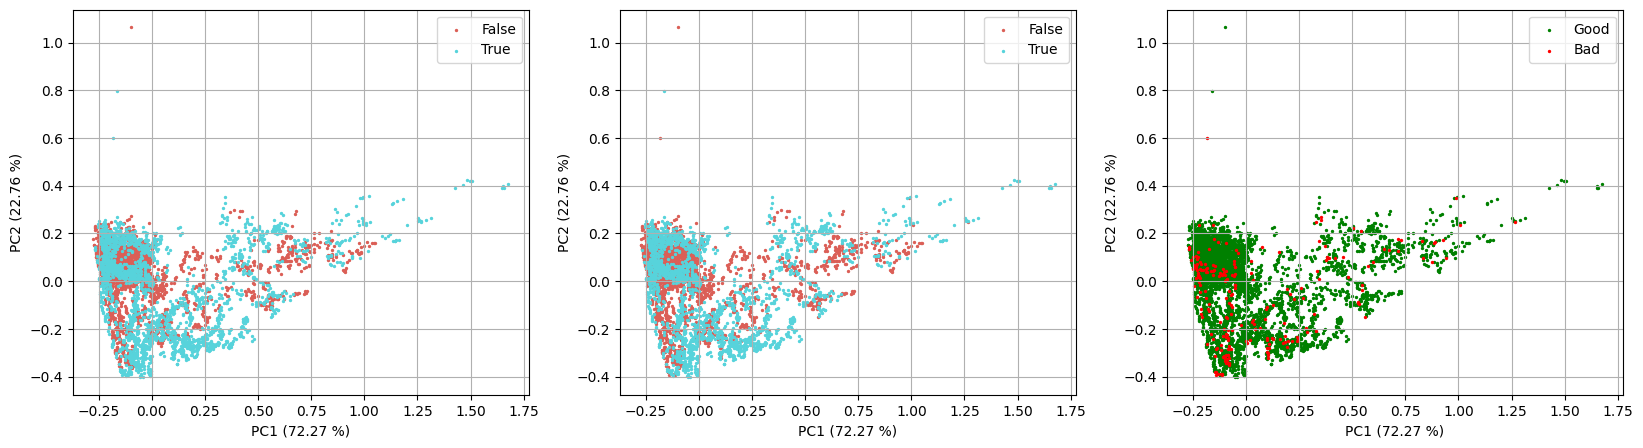
\includegraphics[width=\textwidth]{assets/design/pca-scatter-online-anomaly60-temporal.png}
        \caption{}
    \end{subfigure}
    \hfill
    \begin{subfigure}[b]{\textwidth}
        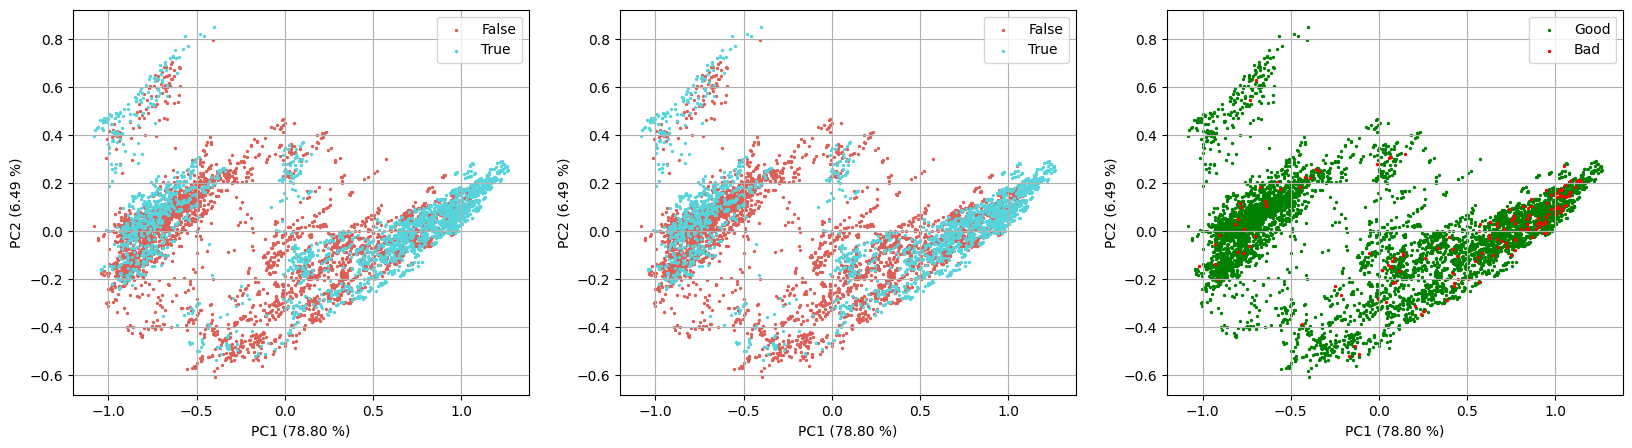
\includegraphics[width=\textwidth]{assets/design/pca-scatter-online-anomaly60-spectral.png}
        \caption{}
    \end{subfigure}
    \caption{PCA 2 components to visualize results and mistakes of online learning on all features}
\end{figure}


\section{Measuments on machinery}
- Machinery
% Enum list

- Sensors

\begin{table}[ht]
\renewcommand{\arraystretch}{1.2}
\begin{tabular}{|l|l|l|}
\hline
\textbf{Accelerometer}                           & \textbf{ADXL335} & \textbf{IIS3DWB}   \\ \hline
\textbf{Vendor}                                  & Analog Devices   & STMicroelectronics \\ \hline
\textbf{Bus}                                     & Analog           & SPI                \\ \hline
\textbf{Axis}                                    & 3                & 1 or 3             \\ \hline
\textbf{Range} (g)                               & $\pm$ 3          & $\pm$ 2 to 16      \\ \hline
\textbf{Bandwidth} (kHz)                         & 0.55             & 5 - 6.3            \\ \hline
\textbf{Sensitivity}                             & 300 mV/g         & 0.061 mg/LSB       \\ \hline
\textbf{Noise density} ($\mu g / \sqrt{\mathrm{Hz}}$ rms) & 150 - 300        & 75                 \\ \hline
\textbf{Microcontroller}                         & Beaglebone Black & ESP32-PoE-ISO      \\ \hline
\textbf{CPU SoC}                                 & TI Sitara AM3358 & ESP32-WROOM-32     \\ \hline
\textbf{Output data rate} (kHz)                  & 2.5              & 26.7               \\ \hline
\textbf{ADC resolution} (bit)                    & 12               & 16                 \\ \hline
\textbf{FIFO}                                    & -                & 3 kB (512 samples) \\ \hline
\end{tabular}
\caption{Accelerometers}
\end{table}

- Preliminary measurements
% Waveforms


\begin{figure}[h]
	\centering
	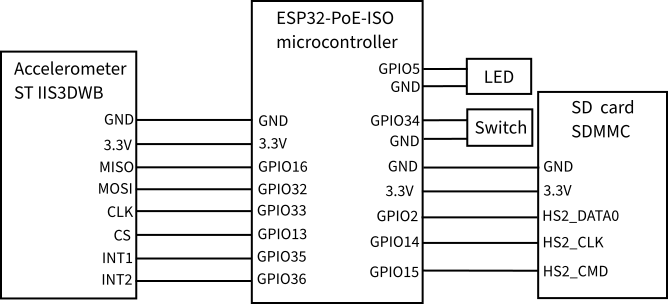
\includegraphics[width=\textwidth]{assets/design/hw-block-schematic.png}
	\caption{Sensor unit hardware block diagram}
\end{figure}


\begin{figure}[ht]
    \centering
    \begin{subfigure}[b]{0.44\textwidth}
        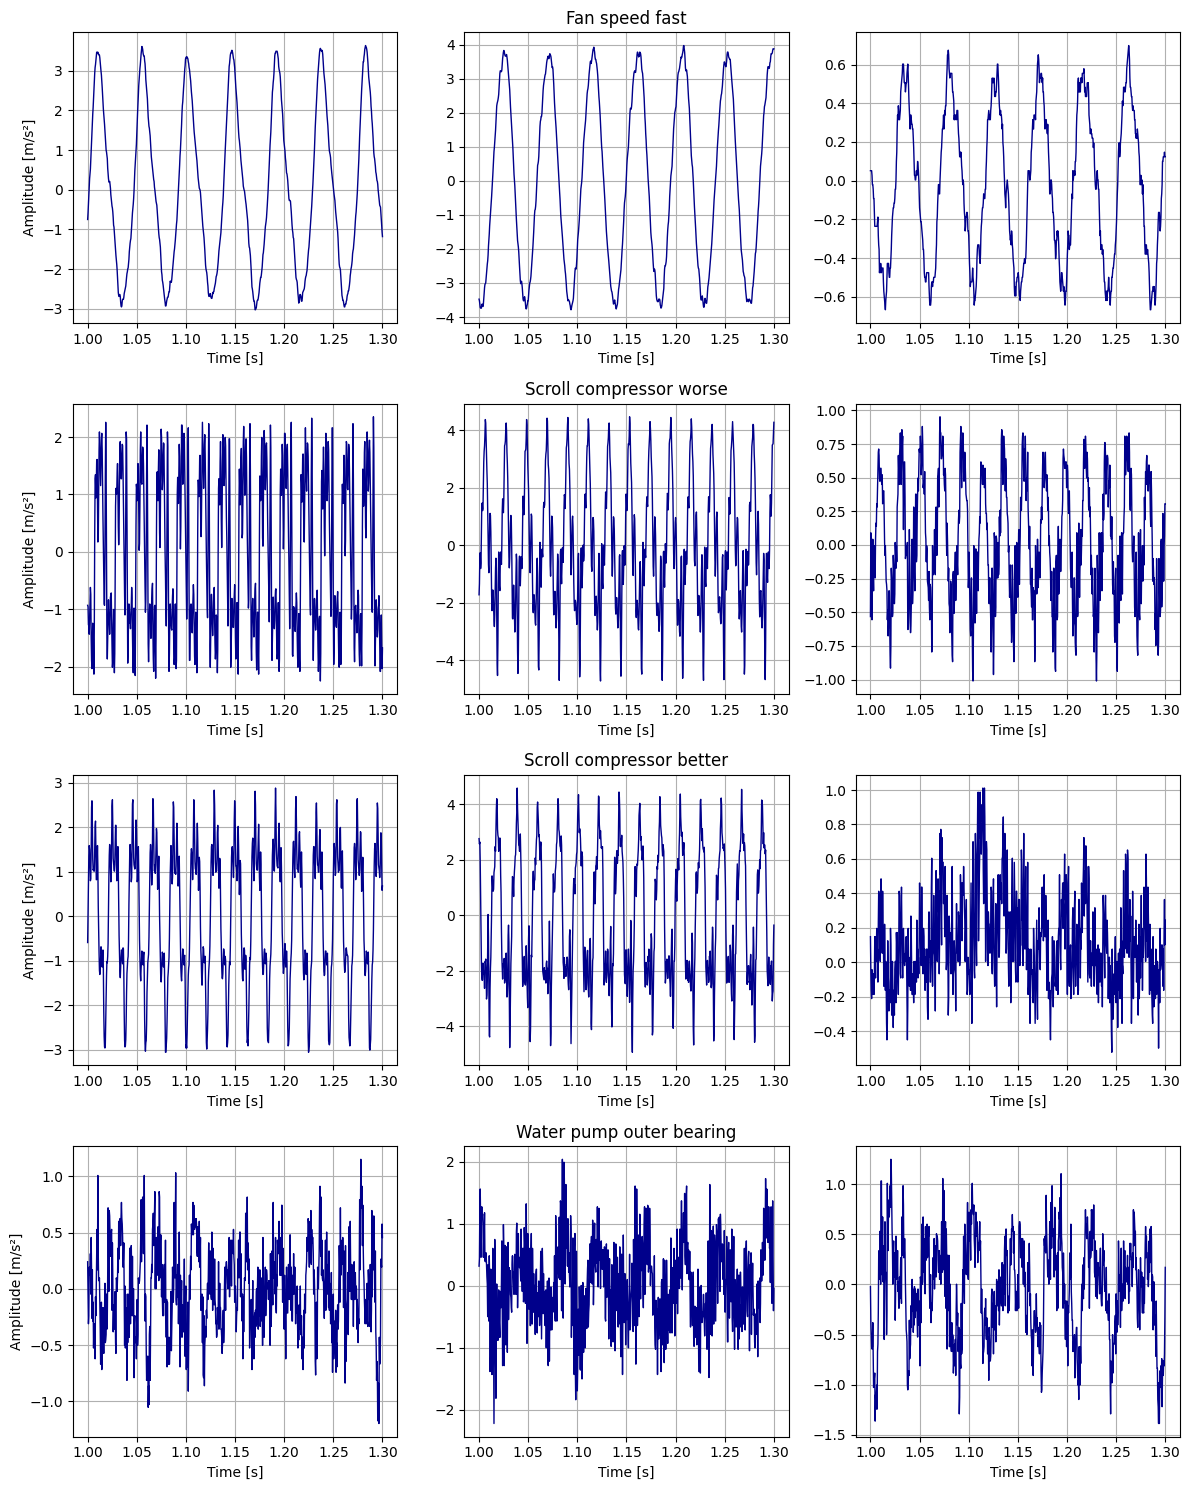
\includegraphics[width=\textwidth]{assets/design/EDA-custom-dataset-temporal.png}
        \caption{Temporal domain waveforms in all spatial directions with 300 ms duration}
    \end{subfigure}
    \hfill
    \begin{subfigure}[b]{0.55\textwidth}
        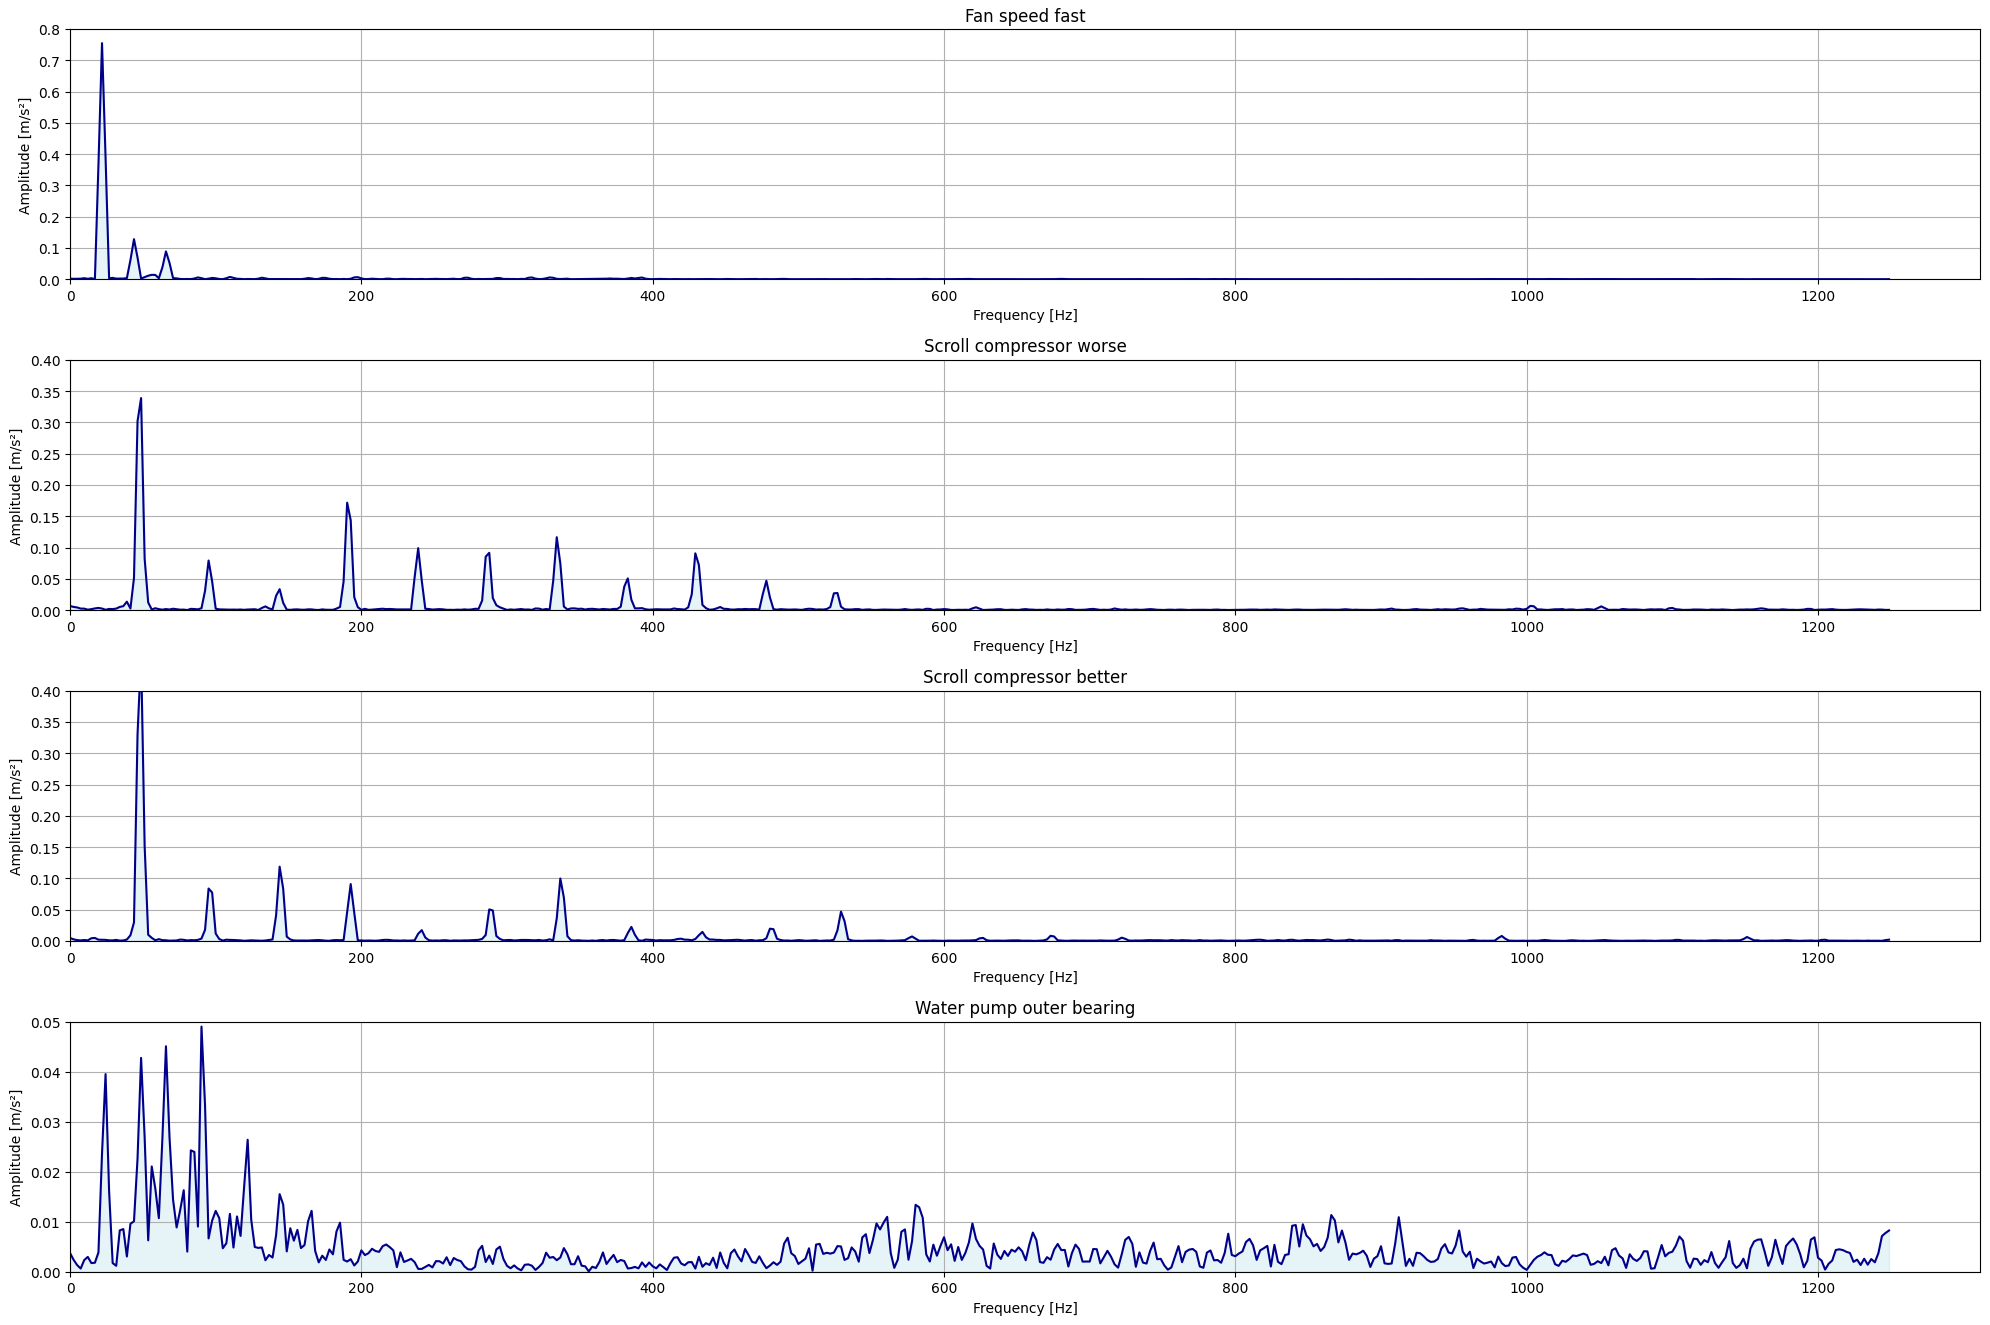
\includegraphics[width=\textwidth]{assets/design/EDA-custom-dataset-spectral-X-axis.png}
        \caption{Spectral domain in x accelerometer axis. FFT with Hann window of length $2^{10}$ ($\approx 409$ ms)}
    \end{subfigure} 
    \caption{Signals at 5 s timestamp}
\end{figure}






\newpage
\section{Machine learning pipeline}
\begin{enumerate}
    \itemsep0pt
    \item Detrending
    \item (Optional) Adaptive noise cancellation of the background interference
    \item Vector of all features
    \begin{itemize}
        \itemsep0pt
        \item Time domain: statistical measures (Tab.~\ref{tab:td-features})
        \item Frequency domain: PSD estimation with FFT and Welch averaging with the resolution of 1 Hz combined with Hann window (Tab.~\ref{tab:fd-features})
    \end{itemize}
    \item Feature selection on evaluation datasets and experimental measurements from the factory to prune away irrelevant features with pearson correlation, Fisher score, and mutal information.
    \item Model evaluation and comparison of novelty detection methods and precision of classification with different sets of predictors. The range of optimal parameters will be found for the DenStream ($\mu$, $\epsilon$, $beta$, $\lambda$), Half-Space Trees (window size, ensemble size), and kNN (distance metric, $k$ neighbours). Evaluation metrics associated with confusion matrices will be used like accuracy, precision, true positive rate, and false positive rate.
\end{enumerate}

\begin{figure}[h]
\centering
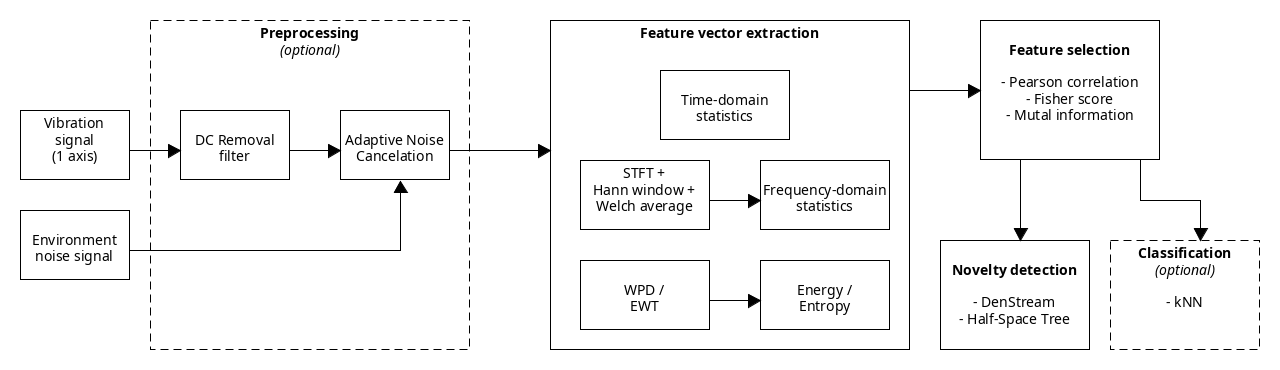
\includegraphics[width=0.9\textwidth]{assets/analysis/ml-lifecycle.png}
\caption{Machine learning lifecycle of feature discovery}
\end{figure}


\section{Data preparation}


- \textbf{Measurements-SHC3.html}
- \textbf{BVS-Measurements.html}

\section{Feature relevance}
- \textbf{FeatureSummary.html}

- choose 3 features
- supervised
	- highly correlated features >= 0.9:
		- Temporal domain (A)
			- std, rms, 1.000000
			- margin, impulse, 0.999079
			- crest, impulse, 0.996807
			- crest, margin,	0.992548
			- pp, max, 0.970055
			- max, (std, rms), 0.938198
			- pp, (std, rms), 0.938180 / 0.928
		- Spectral domain (A)
			- same feature in different window sizes (0.99)
			- kurtosis, skewness, 0.980618
			- std, energy, 0.960110
			- entropy, noisiness, 0.945514

	- calcultate euclidian measure of feature 
	- correlation point biserial, fisher, mutual information
		- Sperman rank correlation: corr, f\_stat, 0.98
	- calculate feature rank
		- Temporal (A) - Remove corr: pp, skewness, margin
		- Spectral (A) - multiple window sizes 
			- (energy, roll off, std) 

- online learning features
	- evolution of feature importace

\section{Nearest neighbour classifier}
- \textbf{kNN.html}
- kNN (fault and anomaly)
	- Offine (baseline)
	- Online (evolution)
- parameters: k-neigh, distance
- metrics: accuracy, precision, recall

\section{Clustering}
- Density based clustering
	- DBSCAN (all features, PCA, subset of best)
	- DenStream (all features, subset of best)

\section{Novelty detection}
- Offline (Isolation forest)
- Online (Half-space Tree)


\section{Infrastructure deployment}
Future work: engineer new feature, deploy, tweek models, validate on real dataset

 \begin{itemize}
 \itemsep0pt
\item \textbf{Input:} Samples from three-axis MEMS accelerometers, RPM tachometer, Noise background
\item \textbf{Output:} machine health status / type of fault
\item \textbf{Output on demand}: Control chart of trend features
\end{itemize}

\begin{enumerate}
\itemsep0pt
\item \textbf{Accelerometer} - MEMS accelerometers will be placed on at least two distinct measurement points in two perpendicular axes and one sensor in the machine base for denoising purposes. Rotational speed has to be captured at the same time too. The sampling frequency shall be around 2 kHz if unbalance and looseness is to be identified, and 10 kHz if bearing faults are also of interest. The range of overall rms vibrations is not expected to exceed 30 mm/s according to the vibration severity chart.
\item \textbf{Acquisition interval} - sensor units will be triggered in regular intervals (every 15 - 60 minutes) to collect vibration recordings from the band saw (or another machine of choice). The machine has to be under the same load conditions every time is recording is active. 
\item \textbf{Features} - most relevant features are computed and compared to recent measurements. If there is a statistically significant change the whole summary is sent, otherwise keep-alive notification is sent. 
\item \textbf{Wireless network} - earlier design decision has been made to establish wireless connections. Therefore, the sensor unit will send data over Wifi (IEEE 802.11), or Thread with IEEE 802.15.4 over 2.4 GHz or 868 MHz frequency bands. The application protocol shall be Constrained Application Protocol (CoAP). The messages will be encoded by Concise Binary Object Representation (CBOR) or MessagePack which provides the best compression ratio and is widely supported.
\item \textbf{Time series database} - stores history of trend values. Raw vibration measurements can be requested by the operator at any time but are available and delayed according to transfer speeds and other network constraints. The promissing database technologies is TimescaleDB.
\item \textbf{Diagnosis panel} - continuously updates the anomaly detection and classification models with the introduction of annotations to notify the operator about observed faults and imminent failure of the machine. The dashboard is provided to display the current status of multiple machines.
\end{enumerate}

\begin{figure}[h]
\centering
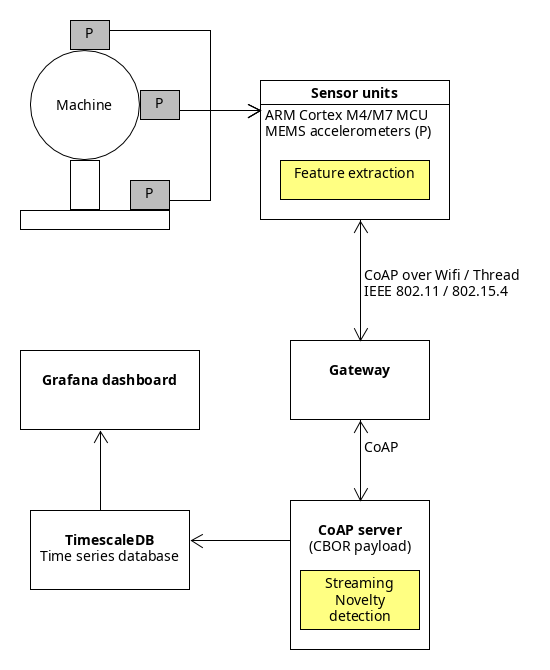
\includegraphics[width=0.7\textwidth]{assets/design/sensor-network.png}
\caption{Sensor network components}
\end{figure}
